%\documentclass[12pt,preprint]{aastex}
%\documentclass[preprint2,12pt]{aastex}
\documentclass{emulateapj}
%\usepackage{apjfonts}
\usepackage{graphicx}
\usepackage{amssymb}
\usepackage{amsmath}
\usepackage{todonotes}
\usepackage{comment}

\shortauthors{LGB, KM, JNW}
\shorttitle{Binary Biases \& Toy Transit Surveys}

\begin{document}

% ------------------------------------------------------------------------
% New commands
%
\def\ltsima{$\; \buildrel < \over \sim \;$}
\def\lsim{\lower.5ex\hbox{\ltsima}}
\def\gtsima{$\; \buildrel > \over \sim \;$}
\def\gsim{\lower.5ex\hbox{\gtsima}}
\def\tess{{\it TESS} }
\def \teff {T_{\rm eff}}
\def \phir {\Phi_{\rm R}}
\def \fov {24$^{\circ}$}
\def \pixsz {21.1''}
\def \aeff {69.1 cm$^2$ }    
\def \epd {105 mm}                          

\def \kepler {{\it Kepler}}

% -------------------------------------------------------------------------
%

\bibliographystyle{apj}

\title{ The Effects of Stellar Binarity on Transit Survey Occurrence 
Rates }

\author{
  LGB, KM, JNW
}

% \journalinfo{Draft version}
\slugcomment{Draft version}

%\altaffiltext{1}{Princeton University}

\begin{abstract}

What errors does ignoring binarity introduce on the occurrence rates derived 
from transit surveys?

\begin{comment}
First, we show that in a universe where all stars have fixed properties
(except that some are twin binaries), the results of a search for planets of a 
given radius and orbital period can be expressed analytically.

We then allow the properties of the secondary in binary systems to vary. A 
distribution of light ratios introduces a detection bias towards 
equal-mass binaries in magnitude limited samples.
We show that dependent upon planet occurrence's functional dependence on host 
star mass, as well as the specifics of the assumed survey completeness, the 
occurrence rate correction factor $X_\Gamma \equiv \Gamma_{\rm 
true}/\Gamma_{\rm obs}$ ranges from $0.6-1.6$.

Finally, we perform a synthetic transit survey analogous to {\it Kepler}. We 
show that if we assume every star in this {\it Kepler} survey analog is single, 
we underestimate occurrence rates for a given planet radius and period by 
a factor of $\approx 1.4$, or a percentage error relative to the true 
occurrence rate $\Gamma_{\rm true}$ of $\delta\Gamma_{\rm 
true}=-28\%$. This is relevant for measuring accurate values of the rate at 
which Earth-like planets exist around Sun-like stars.
\end{comment}


\end{abstract}

\keywords{planets and satellites:\ detection}

\section{Introduction}

An astronomer who does not believe in binaries wants to measure the
occurrence of planets of a certain type around stars of a certain type.
In other words, they wish to find the mean number of planets within specific 
planetary $(R_p, P)$ bounds orbiting the stars in a given volume 
of stellar $(M_\star, R_\star, L_\star)$ phase-space.
They perform a signal-to-noise limited transit survey and detect $N_{\rm det}$ 
transit signals that appear to be from planets of the desired type.  They 
calculate the number of stars $N_\star$ that appear to be searchable for the 
desired type of planet, and also of the desired stellar type.  These 
``searchable stars'' are the points on the sky for which they think planets 
are observed with 100\% detection efficiency. Accounting for the geometric 
transit probability $f_{\rm g}$, they compute an apparent occurrence rate 
$\Gamma_{\rm a}$:

\begin{equation}
\Gamma_{\rm a} = \frac{N_{\rm det}}{N_\star} \times \frac{1}{f_g}.
\end{equation}

There are many potential pitfalls.  Some genuine transit signals can be missed
by the detection pipeline.  Some apparent transit signals are spurious, from
noise fluctuations, failures of `detrending', or instrumental effects.  Stars
and planets can be misclassified due to statistical and systematic errors in
the measurements of their properties.  Poor angular resolution causes false
positives due to blends with background eclipsing binaries. {\it Et cetera}.

Here we focus on problems that arise from the fact that stars of the desired
type often exist in binaries. 
We assume for simplicity that all binaries in the transit survey are 
spatially unresolved.

One immediate complication is that~--~due to dynamical stability or some 
aspect of planet formation~--~ the occurrence rate of planets of the desired 
type may differ between binary and single-star systems.
If ``occurrence rate'' is defined purely as the mean number of planets within 
set radius and period bounds per star in a given interval $\Delta M_\star, 
\Delta R_\star, \Delta L_\star$, it must include an implicit marginalization 
over stellar multiplicity.
Otherwise, one must discuss ``occurrence rates in single star systems'', 
``occurrence rates about primaries of double systems'', and
``occurrence rates about secondaries of double star systems''.

Outside of bonafide astrophysical differences, there are observational biases.
A given apparently-searchable star may truly be a single star of the desired 
type. If not, and ignoring higher order multiples, one of the following must 
be true:
\begin{enumerate}	
\item The apparently-searchable star is a binary system, with two searchable 
stars of the desired type. $N_\star$ is under-counted by one for every such 
system.
%
\item The apparently-searchable star is a binary system, with one searchable 
star of the desired type. 
The searchable star of the desired type could be the primary or the secondary.
$N_\star$ is correctly counted for every such system, though there may be 
systematic errors in estimates of stellar parameters.
%
\item  The apparently-searchable star is a binary system, in which neither of 
the components is a searchable star, but at least one is of the desired type. 
$N_\star$ is over-counted by one for every such system.
\end{enumerate}

One might also imagine an apparently-searchable star which in no stellar 
component is of the desired type.
%For single stars, this may simply be from erroneous stellar parameters.
%In binaries, one might imagine the combined light of two stars somehow making 
%them resemble a single star of the desired type.  
We will not consider errors of this type.  We will assume that all the 
apparently-searchable stars are either single stars of
the desired type, or binaries in which either the primary or else both 
components are of the desired type.

The above enumerates possible errors when counting $N_\star$.
When tallying $N_{\rm det}$, the detected signals from planets of the desired 
type, neglecting binarity introduces the following error cases:
\begin{enumerate}
\item 
A detected signal is from a star of undesired type (by the above assumptions, 
the secondary of a binary system), from a planet of undesired type, and is 
incorrectly counted as a planet of desired type.
%
\item
A detected signal is from a star of desired type (the primary or secondary of 
a binary systems), from a planet of undesired type, and is incorrectly counted 
as a planet of desired type.
This and the case above occur when the host star parameters are miscalculated 
({\it e.g.,} the host star is the faint secondary, but is assumed to be 
primary), or when the constant diluting light from the binary companion is not 
corrected.
$N_{\rm det}$ should be lowered by 1 for every such case.
%
\item
A detected signal is from a star of desired type, from a planet of desired 
type, but incorrectly counted as planet of undesired type.
$N_{\rm det}$ should be raised by 1 for every such case.
\item
An {\it undetected} signal from a planet of the desired type, around a star of 
the desired type, was not detected because of dilution from the companion 
(because the SNR floor of the survey is set for single stars). 
This happens during case \#3 in $N_\star$-counting errors (the 
apparently-searchable star is a binary system, in which neither component is 
in fact searchable). If $N_\star$ is corrected for this, {\it i.e.,} the 
system is correctly counted as ``not searchable'', no correction to $N_{\rm 
det}$ is needed.
\end{enumerate}

Errors (1)-(3) in calculating $N_{\rm det}$ above broadly fall under ``radius 
misclassification'', while error (4) falls under ``completeness 
miscalculation''.
Note that in the above list, a planet cannot be both ``of desired type'' and 
``orbiting a star of undesired type''. We ignore this type of error for 
analytic convenience, but \texttt{reintroduce it later during numerics}.



Our approach is step-by-step starting from a very simple scenario.
\begin{itemize}
\item We consider a universe consisting of only the desired types of stars and
planets.  We give analytic expressions for eta(apparent)/eta(true) taking
into account all applicable errors.
%
\item We allow for a distribution of the mass ratio $dn/dq \propto q^\gamma$, 
and a concurrent power-law distribution in the luminosity ratio, $dn/dL 
\propto L^\beta$. 
%We assume the secondary is not of the desired stellar type.
%NOTE: LB notes that yes, while analytically simple, it doesn't make sense. 
%For the twin binaries case, what possible reason could there be for the 
%secondary to not be of the desired stellar type? Similar for the high mass 
%ratio binaries -- the stars are ~identical.
We give analytic expressions for eta(apparent)/eta(true) taking into 
account errors of type 2.
%NOTE: empirical L(M) maybe OK for numerics -- not for analytics.
%
\item We allow for a nonzero tolerance $\Delta R_p$ in the planet radius, and 
tolerance $\Delta L_\star$ in stellar luminosity, to qualify as "desirable".  
We recalculate eta(apparent)/eta(true).
(LB: I think this has to become numerical to actually evaluate the occurrence
rate correction factor, $X_\Gamma$.)
%
\item We assume the planets have a power-law radius distribution, $d\eta/dR_p
\propto r^\alpha$.  We calculate the apparent $d\eta/dR_p$ taking into account 
errors of type 1-3.  We do so for stars of the desired type within some 
tolerance dL.
%
\item Everything up to now is more-or-less analytic, perhaps supported by 
numerical checking or numerical integration. At the end we summarize the 
radius-dependence of the occurrence rate shifting.
"Accounting only for dilution \& its numerator effect, big radius planets have
underestimated inferred rates, the smallest radius planets have overestimated
inferred rates, and the in-between radius planets are in-between"

\end{itemize}

We then dig in, w/ numerics, to what happens with different assumed
completeness vs Rp functions.
We note that the the claimed HJ occ rate discrepency btwn RV \&
transit surveys gets much weaker when accounting for binarity.
This is b/c the more believable occ rate papers do not heavily rely on their
completeness calibration -- they know they're complete.
This is a much more understandable regime than the wonky completeness estimate 
dependent zone of eta-Earth for Kepler.

Finally, for numerics, we simulate a sample of 20,000 
apparently-searchable-stars (or however many "stars" appear to be searchable
for Earthlike planets in the Kepler field).  Basically this means a magnitude
limited survey of 20,000 ``stars'' that are either single or are binaries with
the primary of the desired type.  The sample has a realistic distribution of
binaries (occurrence and luminosity ratio).  We calculate 
eta(apparent)/eta(true).  We can also play with errors of type 4 in this
numerical model (i.e. we let the relative occurrence rates between primaries 
and secondaries vary).  (It may not worth doing so for the analytic 
work-- though it's pretty simple. The way to play with this is just present 
both limits, and then also present a few weight factors (Furlan+17 do a good 
job).


We discuss ``how do we interpret Fulton+ 2017?''
That paper did (or claims to have done) a good job at weeding out numerator
errors. If true, means $\Gamma(R_{\rm p})$ has the right shape, and just the 
wrong normalization. Important if we ever manage to convince ourselves 
``brightest transit hosts'' could work.

In passing, at the end, we mention how this changes attempts at eta-Earth 
measurements.


\begin{comment}
UNSOLVED PROBLEMS W/ THE NUMERICAL MODEL-
* currently have not implemented self-consistent (L,M,R) relation between
primaries and secondaries.
Wang et al (2015) avoided that problem by doing a similar empirical thing to
what I currently have implemented. But I do not think that was a good paper.
Ciardi et al (2015) have an approach that was Kepler-specific -- they used
the same Dartmouth isochrones used for KIC stellar parameters.
But they did not conserve $dn/dm_x$, for $m_x$ apparent mag in band x.
I think the latter choice might be better for Kepler-specific discussion.
But it's less-nice if we want this to be general enough for e.g., occ HJ
rates w/ TESS.

My main gripe w/ taking the 150k KIC stars \& adding binaries is that less
is known about those parameters and biases. Using e.g., Galaxia has the major
benefit of you understand what's been cooked in much better (it's minimal).

I think if we want to talk about Kepler, it's the best possible approach
though.

If we want to talk about Fulton+17 we can go further, and apply the CKS cuts.


Some questions based on the current draft:

- Why should we ever consider $F_{lim} < F_{min}$?

LB: in practice, surveys look at many stars for which they could not detect
Rp=Re planets, but could detect Rp=10Re planets.  One possible error is
miscounting which stars are which (i.e. getting completeness corrections
wrong). So this was more for plausbility than b/c it's immediately needed in
the analytics. I can cut it.

- Why do we need to consider the distribution of S/N, as opposed to simply the
limiting distance for detection?

LB: for "model 1" (fixed stars, fixed planets, fixed light ratio binaries)
you're correct, it's not immediately necessary. 

For this model, I did it as a way to think through the completeness effects
systematically -- i.e. how for the twin-binary case, you get a completeness
fraction of 1/8, though your limiting distance is sqrt(2) times bigger. (Even
when your completeness for the singles is 100%).

If we go the path of completing "model 2"'s analytics (vary light ratio, fixed
primary luminosity, fixed planet), I think this formulation would become
necessary in order to actually evaluate the completeness fractions.

(I never completed these analytics b/c of the L(M) mess + confusion about
assumed stellar masses+radii. Power law L(M) helps this... I think there needs
to be an extra assumption about the stellar mass+radius change though that we
have not spelled out)

- I don't think the bandpass, effective area, photon count rate, etc.  are
needed, either. All that matters is the limiting distance.

Are needed for what? 
In Model 1, for analytic expressions of the occurrence rate, I agree.
For analytic expressions of the number of detected planets, I disagree.

For Model 2, I'm not sure because I got bogged down. I suspect that for
occurrence rate errors, you are correct. 

The analytic expression I gave for the occurrence rate depends on this "xi"
factor, which needs to incorporate an assumption about how Astronomer A
misestimates the completeness (relatedly, how he misestimates Rstar).  I never
specified that assumption.


- In Eq. 4, is this a traditional definition of BF?  I would have defined it as
nd/(ns+nd) or perhaps 2*nd/(ns+ 2*nd).  Let's make sure we are using
traditional terminology, and also interpreting the literature correctly, i.e.,
is the right number really 0.45?

Oops. nd/(ns+nd) = BF = MF (if assuming all multiple systems are binaries).
This minor change propagates.

Touching up on correct terminology, from Duchene \& Kraus 2013, Sec 2.1:

"Frequency of multiple systems" (MF)
vs
"Companion frequency" (CF; average \# of companions per target, can exceed 
100\%)

my understanding of the terms:

survey 1: {*, **, *, ***, *, *}

6 systems.
2 are multiple.
MF = 2/6 = 1/3
CF = (0+1+0+2+0+0)/6 = 3/6 = 1/2

survey 2: {**, **, ***, ****, *}

5 systems
4 are multiple
MF = 4/5
CF = (1+1+2+3+0)/5 = 6/5

DK2013 Sec 3.1.1 give (citing Raghavan+ 2010)
MF^{MS}_{1-1.3Msun} = 50 \pm 4%
MF^{MS}_{0.7-1Msun} = 41 \pm 3%

They also give
CF^{MS}_{1-1.3Msun} = 75 \pm 5%
CF^{MS}_{0.7-1Msun} = 56 \pm 4%

I understand the first pair of numbers to mean:

In a volume-limited survey (of the stellar neighborhood), if you select systems
for which the primary is from 1-1.3Msun, 50% of them will be multiple.

I take the second pair of numbers to mean:

In a volume-limited survey (of the stellar neighborhood), if you select systems
for which the primary is from 1-1.3Msun, each system will on average have 0.75
companions.

So YES, need to correct this throughout.
\end{comment}





\section{Model \#1: fixed stars, fixed planets, fixed light-ratio binaries}
\label{sec:model_1}

Stellar binarity introduces convoluted effects on transit surveys.
To disentangle them, imagine the following idealized survey.

You observe the entire sky for some duration with a detector of known 
area and bandpass. Your detector is photon-noise limited.
You are interested only in detecting planets of radius $R_p$, and orbital 
period $P$. For instance, $R_p=R_\oplus$, $P={\rm 1\ year}$.
You are only interested in detecting them around stars of radius $R_1$, 
and luminosity $L_1$. For instance, G2V dwarfs.
You can only detect your desired type of planet when you observe signals 
with ${\rm S/N} > {\rm (S/N)_{min}}$.
For a photon-noise limited survey, this minimum signal to noise ratio is 
equivalent to a minimum flux required for detection, $F_{\rm min}$.

You get funding, and perform the S/N-limited survey. 
You observe all the ``points'' on-sky with apparent 
magnitude $m < m_{\rm min}$, or equivalently with energy flux in your bandpass 
greater than some limit $F > F_{\rm min}$.
All planets with ${\rm S/N} > {\rm (S/N)_{min}}$ are detected. The rest are 
not.

You now wish to derive an occurrence rate for planets of radius $R_p$ and 
orbital period $P$.
Assume your universe is a universe in which:
\begin{itemize}
	\item The true population of ``points'' (stellar systems, all unresolved) 
	comprises only single and double star systems. Single star systems have 
	luminosity in the observed bandpass $L_1$, radii $R_1$, and effective 
	temperature $T_{\rm eff,1}$.
	Double star systems have luminosity in the observed bandpass $L_d = 
	(1+\gamma_R)L_1$, for $\gamma_R = L_2/L_1$ the ratio of the luminosity of 
	the secondary to the primary. 
	In this section, $\gamma_R=1$ across the population 
	of star systems~--~all binaries are assumed to be twin systems.
	The ratio of the number density of binary systems and the number density of 
	all systems in a volume-limited sample is the binary fraction\footnote{The 
	binary fraction is equivalent to the multiplicity fraction if there are 
	no triple, quadruple, $\ldots$ systems.}.
	\item The true population of planets around these stars is as follows:
	\begin{itemize}
	\item A fraction $\Gamma_{t,s}$ of stars in single star systems 
	have planets of radius $R_p$, with orbital period $P$.
	\item A fraction $\Gamma_{t,d}$ of primary stars in double star 
	systems have planets of radius $R_p$, with orbital period $P$. 
	A fraction $w_{d2}\Gamma_{t,d}$ of secondary stars in a double star 
	systems have the same type of 
	planet, where the weight factor $w_{d2}$ specifies the secondary star 
	occurrence rate as a fraction	of the primary star occurrence rate.
	Any astrophysical difference in planet formation between singles and 
	binaries is captured by $\Gamma_{t,s}, \Gamma_{t,d},$ and $w_{d2}$.
	If one assumes the primary and secondary of a binary system host planets at 
	equal rates, this is the $w_{d2}=1$ limit.
	Similarly, if one assumes  secondaries 
	cannot host planets, this is the $w_{d2}=0$ limit.
	\end{itemize}
\end{itemize}

The assumption of [Pepper et al, 2003] in a very similar context was that the 
observer correctly pre-selects all of the ``searchable stars''.
This simplification would allow the observer to ignore 
completeness effects when deriving occurrence rates, since their completeness 
is 100\%.

The above approach ignores incompleteness for binary systems.
If we set the limiting flux to give 100\% completeness for single stars, we 
will unwittingly select binaries near that flux limit, for which dilution 
will push transit signals below the detection threshold.
This is because a flux limit maps onto three distinct maximum 
detection distances for a population of single stars and twin binaries:
\begin{enumerate}
\item $d_{{\rm max},s}$: the maximum distance out to which the desired type 
	of planet is detectable around single stars.
	These are the selected ``searchable, single stars''.
%
\item $d_{{\rm max},d}$: the maximum distance out to which double stars
  are selected (down to the same minimum flux as that defining $d_{{\rm 
  max},s}$). 
  This is different from $d_{{\rm max},d}^{\rm p}$, the maximum
  distance out to which planets are detectable around double stars. For a 
  population with fixed  $\gamma_R$, since ${\rm S/N} \propto \mathcal{D} 
  L^{1/2} d^{-1}$,
  \begin{equation}
    d_{{\rm max},d}^{\rm p} = (1 + \gamma_R)^{-1/2} d_{{\rm max},s} = 
    (1 + \gamma_R)^{-1} d_{{\rm max},d}.
  \end{equation}
  For $\gamma_R = 1$, this means only 1 in 8 apparently-searchable stars which 
  are in fact binary systems can yield detectable planets (the ratio of 
  volume in which planets can be detected to the actual selected volume).
  For a more realistic sample, $\gamma_R \approx 0.1$, and there is an 
  interesting asymmetry.
  One finds the completeness for planets which orbit the primary star, 
  $f_{d1,c}$ to be
  \begin{equation}
  f_{d1,c} = (1+\gamma_R)^{-3} \approx 3/4.
  \end{equation}
  However, for planets which orbit the secondary star, the completeness is
  \begin{equation}
    f_{d2,c} = (1+\gamma_R^{-1})^{-3} \approx 3/4000.
  \end{equation}  
  
\end{enumerate}

We note in passing that we are considering a SNR-limited survey, which in this 
case is the same as a magnitude-limited one.
The observer might prefer to perform a completeness-limited survey, which in 
this case would be the same as a volume-limited one with limiting distance
$d_{{\rm max},d}^{\rm p}$.
This change would likely improve interpretability.

With the stage set, we ask:

\subsection{What is the true occurrence rate?}
\label{sec:true_rate}

The ``true occurrence rate'' $\Gamma_t$ is the average number of planets of 
the desired type per star of the desired type:
\begin{align}
\Gamma_t &= \frac{N_{\rm planets}}{N_{\rm stars}} \\
\Gamma_t &= \frac{\Gamma_{t,s} N_s + (1+w_{d2}) \Gamma_{t,d} N_d}{N_s + 2N_d}.
\label{eq:true_occ}
\end{align}
where $N_s$ is the number of single star systems, and $N_d$ the number of 
double star systems. 
The factor of 2 in the total number of stars accounts for the fact that there 
are twice as many stars in double star systems.

To develop more analytic expressions in terms of observables, assume that the 
stars are homogeneously distributed\footnote{
If we wished to write a stellar number density profile that accounted for the 
vertical structure of the Milky Way, we might choose a profile either $\propto 
\exp(-z/H)$, or $\propto {\rm sech}^2(z/H)$ for $z$ the distance from the 
galactic midplane and $H$ a scale-height. Both density profiles would lead 
closed form analytic solutions.	}.
Counting the number of single and double systems in their respective selected 
volumes,
\begin{equation}
N_i = n_{i} \frac{4\pi}{3} d_{{\rm max},i}^3,
\label{eq:number_systems}
\end{equation}
for $i\in{\rm \{single,double\} } \equiv { \{s,d\} }$, and
\begin{equation}
\frac{n_{d}}{n_s+n_d} = {\rm binary\ fraction} \equiv {\rm BF}
\end{equation}
The absolute normalization of the number density $n_s + n_d$ is an observed
quantity [Bovy 2017], as is the binary fraction.
For ``sun-like'' dwarfs with $0.7<M_\star/M_\odot<1.3$,
${\rm BF}=0.44\pm0.02$ [Duchene \& Kraus, 2013, Raghavan et al 2010]. 
Note that these latter authors really quote a {\it multiplicity} fraction of
0.44 for sun-like dwarfs~--~we count the $\approx 25\%$ of multiple 
systems that are higher order multiples as doubles.

$d_{{\rm max},i}$ in Eq.~\ref{eq:number_systems} is the maximum distance 
corresponding to the given magnitude limit:
\begin{equation}
d_{{\rm max},i} = \left(\frac{L_{i}}{4 \pi F_{{\rm min}}}\right)^{1/2},
\label{eq:d_max}
\end{equation}
where the limiting flux in the bandpass $F_{{\rm min}}$ could equivalently be 
stated in terms of a limiting magnitude $m_{{\rm min}}$.
In Eq.~\ref{eq:d_max}, again $i\in{\rm \{single,double\} }$. Simply as a 
consequence of imposing a magnitude cut, the maximum distance to which binary 
stars will be selected is greater than that of single stars.
The ratio of double to single systems in the observed SNR-limited sample is 
then
\begin{align}
\frac{N_d}{N_s} &= 
	\frac{n_d}{n_s}
	\left( \frac{d_{{\rm max}, d} }{d_{{\rm max}, s}} \right)^3 \\
&= \frac{{\rm BF}}{1 - {\rm BF}} \times (1+\gamma_R)^{3/2}.
\end{align}
In the case of twin binaries ($\gamma_R = 1$), with a binary fraction 
${\rm BF} = 0.5$, there are 
$2^{3/2}\approx2.8$ times more binary systems than single systems in the 
SNR-limited sample.
Since the completeness fraction for binary systems is $1/8$, there are 
$2^{-3/2}\approx0.35$ times fewer binary systems in the sample that can yield 
planets as single star systems in the system that can yield planets.




\subsection{What is the measured occurrence rate?}
% % % % % % % % % % % %

The observer who has never heard of binary star systems wants to find the 
occurrence rate of planets with radius $R_p$ and period $P$, orbiting stars of 
radius $R_1$ and luminosity $L_1$.
They detected $N_{\rm det}$ transit signals that appear to be from planets of 
this desired type.
The occurrence rate they then find, {\it i.e.} the number of planets divided 
by number of ``stars'' (really, stellar systems) is
\begin{equation}
\Gamma_{\rm a } = \frac{N_{\rm det}}{N_s + N_d} \times \frac{1}{f_g}.
\end{equation}

Since only the transit depth is observed, the planetary radii apparent to this 
astronomer, $R_{\rm p, a}$, are different from the true planetary radii 
$R_{\rm p, t}$. 
This is because the assumed stellar radii $R_{\star,{\rm a}}$ may differ from 
the true stellar radii $R_{\star,{\rm t}}$, and the flux will be diluted:
\begin{equation}
R_{p,{\rm a}} = R_{p,{\rm t}} 
\frac{R_{\star,{\rm a}}}
		 {R_{\star,{\rm t}}}
		 \,\mathcal{D}^{1/2},
\end{equation}
where the dilution parameter $\mathcal{D}$ is defined for binary systems as
\begin{align}
\mathcal{D} &= 
\Bigg\{\begin{array}{lr}
L_1 / L_d, & \text{if\ planet\ orbits\ primary}\\
\gamma_R L_1 / L_d, & \text{\ if\ planet\ orbits\ secondary}
\end{array} \nonumber\\
&=
\Bigg\{\begin{array}{lr}
(1+\gamma_R)^{-1}, & \text{if\ planet\ orbits\ primary}\\
(1 + \gamma_R^{-1})^{-1}, & \text{if\ planet\ orbits\ secondary}
\end{array} 
\label{eq:dilution}
\end{align}
where $L_1, L_d,$ and $\gamma_R$ were defined in the opening monograph.


In our twin binary thought-experiment, dilution means that all planets 
detected in binary systems will have apparent radii of $R_p/\sqrt{2}$.
Since for twin binaries the stellar radii are the same, the transit 
probability will be correctly calculated.

The total number of planet detections, irrespective of whether they are ``of 
the desired type'', is the sum of the number of planets 
detected in single star systems $N_{{\rm det},s}$ and the number of planets 
detected in double star systems $N_{{\rm det},d}$.
Expressing each individually,
\begin{equation}
N_{{\rm det},s} = N_s \Gamma_{t,s} f_{s,g} f_{s,c},
\label{eq:N_det_s}
\end{equation}
where the product $N_s \Gamma_{t,s}$ is the number of planets in the single 
star systems of the sample, $f_{s,g}$ is the geometric transit probability, 
and $f_{s,c}$ is the fraction of these transiting planets that are observed 
with signal to noise greater than the minimum detection threshold (the 
completeness). 
For our SNR-limited, twin-binary survey, $f_{s,g} = R_1/a\equiv f_g$, and 
$f_{s,c}=1$.

Analogously,
\begin{equation}
N_{{\rm det},d} = (1+w_{d2}) N_d \Gamma_{t,d} f_{d,g} f_{d,c},
\label{eq:N_det_d}
\end{equation}
where now $(1+w_{d2}) N_d \Gamma_{t,d}$ is the number of planets in the double 
star systems of the sample, the geometric transit probability $f_{d,g}=R_1/a$ 
for our twin-binary survey, and $f_{d,c}=1/8$ by the geometric argument 
presented in the initial discussion of limiting distances.

The occurrence rate this astronomer derives for planets of assumed 
radius $R_p$ orbiting stars thought to be of the desired type is then
\begin{equation}
\Gamma_{\rm a} = \frac{\Gamma_{t,s}N_s}{N_s + N_d}.
\end{equation}


\subsection{Errors on derived occurrence rates for twin-binary thought 
experiment}
The ratio of the true to calculated occurrence rates for planets of radius 
$R_p$, $X_\Gamma$, is
\begin{align}
X_\Gamma &=
\frac{\Gamma_t}{\Gamma_{\rm a}} \\
&=
\frac{\Gamma_{t,s}N_s + (1+w_{d2})\Gamma_{t,d}N_d}{\Gamma_{t,s} N_s } \cdot 
\frac{N_s + N_d}{N_s + 2N_d} \\
&= 
\left( 
1 + \frac{(1+w_{d2}) \Gamma_{t,d}}{\Gamma_{t,s}} \beta
\right) \cdot 
\frac{1+\beta}{1+2\beta},
\end{align}
for
\begin{equation}
\beta \equiv N_d/N_s = \frac{\rm BF}{1- {\rm BF}} \times (1+\gamma_R)^{3/2}.
\end{equation}

For the nominal G2V dwarf case of ${\rm BF}=0.44$, if we assume that all stars 
have equal occurrence rates, $\Gamma_{t,s} = \Gamma_{t,d}$ and 
$w_{d2}=1$, then we find $X_\Gamma = 1+\beta = 1+ 2^{3/2}\approx4$~--~ the 
observed occurrence rate is underestimated by a factor of 4.


For the planets around double stars with observed radii $R_p 
\sqrt{\mathcal{D}}$, there is also the error of their misclassification.
The fraction of detections with misclassified radii can be written
\begin{equation}
\frac{N_{\rm det,d}}{N_{\rm det,s} + N_{\rm det,d}} = \frac{1}{1+\zeta},
\end{equation}
for
\begin{equation}
\zeta \equiv \frac{N_s \Gamma_{t,s} f_{s,g} f_{s,c}}{
	 (1+w_{d2})N_d \Gamma_{t,d} f_{d,g} f_{d,c }}.
\end{equation}

For our nominal G2V dwarf case, the twin binaries with equal 
occurrence rates gives $\zeta = 4/\beta = \sqrt{2}$, so 41\% of detections 
have misclassified radii, all of $R_p/\sqrt{2}$.

Of course more generally, the observer might define their 
desired ``type of planet'' to be anything within some margin of $R_p$.
Considering this for the idealized twin-binary case, if the margin includes 
the planets in binary systems, the number of detections ``of the desired 
type'' would change.
The correction factor $X_\Gamma$ would then become
\begin{equation}
X_\Gamma = 
\frac{\Gamma_{t,s} + (1+w_{d2})\Gamma_{t,d}\beta}{\Gamma_{t,s} + 
(1+w_{d2})\Gamma_{t,d} f_{d,c} } \cdot 
\frac{1+\beta}{1+2\beta},
\end{equation}
which simplifies to $(1+2f_{d,c})^{-1} (1+\beta) = 4(1+\beta)/5\approx 3$ for 
our twin-binary thought experiment.
This makes sense: increasing the radius interval of ``desired planets'' 
decreases the error in the numerator, but the error of mis-counted stars in 
the denominator remains identical.


\section{Model \#2: fixed primaries, fixed planets, varying light-ratio 
secondaries}
\label{sec:model_2}

The model of Sec.~\ref{sec:model_1} is idealized, but it helps
develop intuition.
Now, we let the light ratio $\gamma_R = L_2/L_1$ vary across the population 
of star systems.
It does so because the underlying mass ratio $q=M_2/M_1$ varies.
We keep the primary mass fixed as $M_1$, which is also the mass of all single 
stars.

One parametrization for the distribution of 
binary mass ratios in a volume-limited sample is $f(q)\propto q^\gamma$.
[Duchene and Kraus 2013], fitting all the multiple systems of [Raghavan et al 
(2010)]'s Fig 16, quote $\gamma = 0.28\pm0.05$ for $0.7<M_\star/M_\odot<1.3$.
Examining only the binary systems of Rhagavan et al 2010, Fig 16, the 
distribution is roughly uniform,
\begin{equation}
{\rm prob}(q) =
\Bigg\{\begin{array}{lr}
c_q & 0.1 < q \leq 1  \\
0 & {\rm otherwise},
\end{array}
\label{eq:mass_ratio}
\end{equation}
provided we ignore the peak at high mass ratios for analytic convenience. $c_q 
= 1/9$ is the normalization.
We choose this latter mass ratio distribution.

For the mass-luminosity relation, for analytic convenience we assume 
$L \propto M^\alpha$, with the lore-value of $\alpha$ being $3.5$.
As a simple check, we fit lines to mass-luminosity data\footnote{
    Data collected by Torres et al. [2009] for dwarfs earlier than 
    spectral class M, and Benedict et al. [2016] for dwarfs later than 
    spectral class M.
    To convert Benedict et al. [2016]'s reported $M_V$ values to absolute 
    luminosities, we interpolated over E. Mamajek's 
    table
	\texttt{pas.rochester.edu/\textasciitilde 
		emamajek/EEM\_dwarf\_UBVIJHK\_colors\_Teff.txt},
	downloaded 2017.08.02}.
In log-log space, we let the intersection point of the lines float. The 
resulting fit parameters are available in a footnote\footnote{
	m lo: 1.8818719873988132~--~
	c lo: -0.9799647314108376~--~
	m hi: 5.1540712426599882~--~
	c hi: 0.0127626185389781~--~
	M at merge: 0.4972991257826812~--~
	L at merge: 0.0281260412126928.
}. Though the data show a break at $M_\star \approx 0.5M_\odot$, the 
$L=M^{3.5}$ relation is a reasonable fit for $M\lesssim 2M_\odot$.

The final addition to our model is that we must assume a stellar mass-radius 
relation.
This affects the transit probabilities and signal sizes about the 
secondaries of binary star systems.
Since again, our main purpose is to develop intuition about observational 
biases, we approximate this as 
\begin{equation}
R\propto M.
\end{equation}
\begin{comment}
[Demircan \& Kahraman 1991]'s empirical fit to eclipsing 
binary data,
\begin{equation}
R = 1.06 M^{0.945}
\label{eq:mass_radius}
\end{equation}
applies for all the stars in our desired mass range ($M < 1.66M_\odot$, D\&K 
1991's stated bounds), where each quantity is given in solar units. 
\end{comment}

In passing, we note that while $w_{d2}=1$ was a reasonable assumption in 
Sec.~\ref{sec:model_1} (since secondaries were identical to primaries), in 
binary systems we now have secondaries with different stellar properties from 
primaries.
Recall that our occurrence rate is defined for planets of a given type 
orbiting stars of a given type.
Assume our universe is one in which the primary mass of all stars is 
$M_1=M_\odot$.
If this is the case, we might define our ``stars of interest'' to be 
those with $0.7<M_\star/M_\odot<1.3$.
Then, in a volume-limited sample, 1 in 3 secondaries would be ``of interest'', 
and could contribute to the true occurrence rate.
The general point is that $w_{d2}$ will be less than 1, unless planets of the 
desired type are more common around secondaries of lower mass (as may actually 
be true for small planets around M dwarfs).
Keeping this in mind, we ask the same questions as for Model \#1.

\subsection{What is the true occurrence rate?}

The true occurrence rate is the average number of planets of the desired type 
per star of the desired type.
The number of planets of the desired type is
\begin{equation}
N_{\rm planets} = \Gamma_{t,s}N_s + \Gamma_{t,d}N_d + 
\Gamma_{t,d}w_{d2}f_{{\rm desired}}N_d,
\end{equation}
where as before $N_s$ and $N_d$ are the number of single and double systems, 
and the fraction $f_{{\rm desired}}$ is defined so that $f_{{\rm desired}} 
N_d$ is the number of secondaries that are of the desired type, and as before 
$\Gamma_{t,d}w_{d2}$ is the average number of planets each of these desired 
stars hosts.

Counting the number of desired stars, $N_s$ is the same as in 
Sec.~\ref{sec:model_1}. However
\begin{equation}
N_d(\gamma_R) = n_d \frac{4\pi}{3} d_{\rm max,d}^3
\end{equation}
for
\begin{equation}
d_{\rm max,d} =
d_{\rm max,s}\times (1+\gamma_R)^{1/2},
\end{equation}
where $d_{\rm max,s}$ is given by Eq.~\ref{eq:d_max}.

For a given binary system, $q$, $\gamma_R$, and thus $d_{\rm 
	max,d}(\gamma_R)$ are all random variables.
Since $N_d$ is a function of $d_{\rm max,d}$, 
the number of double star systems becomes a random variable, drawn from the 
ensemble of all possible transit surveys.
Applying the chain rule for probability density functions, the distribution 
function for the number of binary systems,
${\rm prob}(N_d)$, can be written 
\begin{equation}
{\rm prob}(N_d) = {\rm prob}(q(\gamma_R)) 
\left| \frac{{\rm d}q}{{\rm d}\gamma_R}  \right|
\left| \frac{{\rm d}\gamma_R}{{\rm d}d_{\rm max,d}}  \right|				
\left| \frac{{\rm d}d_{\rm max,d}}{{\rm d}N_d}  \right|.
\label{eq:prob_Nd_raw}
\end{equation}

\paragraph{Necessary aside on biases in mass ratio distributions}

\begin{figure}[!t]
	\begin{center}
		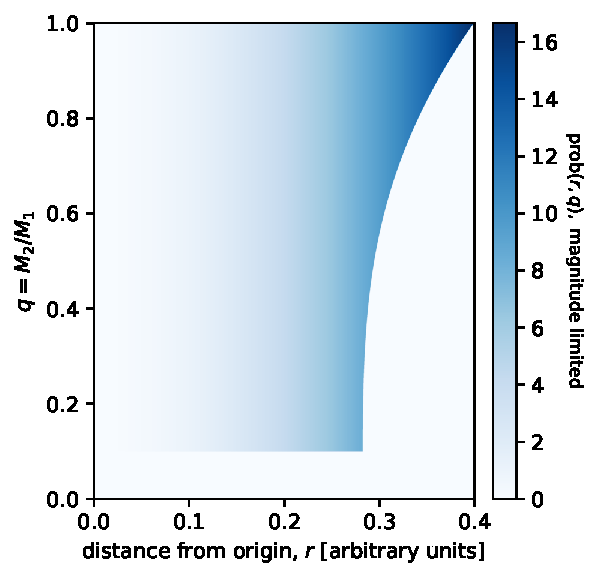
\includegraphics[scale=.8]{figures/joint_prob_r_q.pdf}
	\end{center}
	\caption{The joint probability distribution of a binary star's position and 
		mass ratio in a magnitude-limited sample. This plot assumes $L\propto 
		M^{3.5}$. Note that the marginalized 
		mass ratio distribution is uniform at any given distance.}
	\label{fig:joint_prob_r_q}
\end{figure}

\begin{figure}[!t]
	\begin{center}
		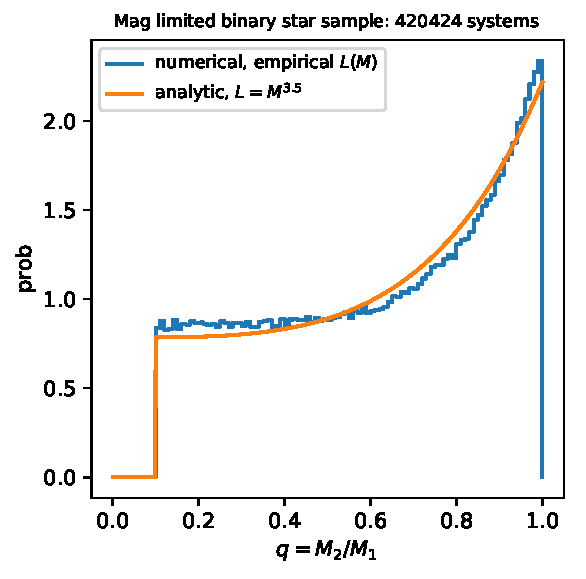
\includegraphics[width=0.5\textwidth]{figures/q_distribn_mag_limited.pdf}
	\end{center}
	\caption{The distribution of the mass ratio for a magnitude limited 
		sample of binary stars. The underlying mass ratios are drawn from 
		Eq.~\ref{eq:mass_ratio} -- a \textit{uniform} distribution in a 
		volume-limited sample.
		The entire bias can be understood analytically 
		(Eq.~\ref{eq:pdf_q_mag_limited}) to good precision. 
        The numerical comparison uses the empirical mass-luminosity relation 
        shown in Fig.~\ref{fig:mass_luminosity}.
	}
	\label{fig:q_distribn_mag_limited}
\end{figure}

\begin{figure}[!t]
	\begin{center}
		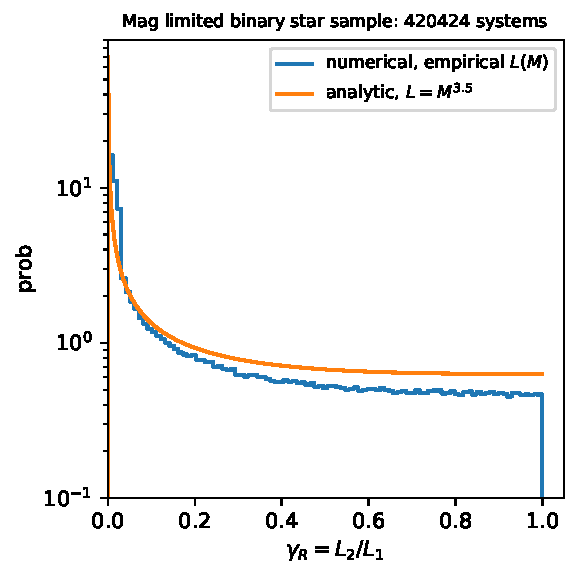
\includegraphics[width=.5\textwidth]{figures/gammaR_distribn_mag_limited.pdf}
	\end{center}
	\caption{The distribution of the luminosity ratio for a magnitude limited 
		sample of binary stars. Despite the preference in the sample towards 
		large $q$ binaries (Fig.~\protect\ref{fig:q_distribn_mag_limited}), 
		the bias is towards small $\gamma_R$ binaries because of the steepness 
		of the mass-luminosity relation.
        The underlying mass ratios are uniform in volume.
        The numerical comparison uses the empirical mass-luminosity relation 
        shown in Fig.~\ref{fig:mass_luminosity}.       
    }
	\label{fig:gammaR_distribn_mag_limited}
\end{figure}


Before blindly plugging in Eq.~\ref{eq:mass_ratio}'s assumed mass ratio 
distribution to find the expected number of double systems, we must
emphasize that Eq.~\ref{eq:mass_ratio}'s distribution applies only for 
volume-limited samples.
If one is interested in a SNR-limited transit survey (or really any
magnitude-limited survey), the Malmquist-like bias associated with binarity
must be included.

The distribution function for the mass ratio of binaries in a magnitude 
limited sample can be found by marginalizing over the joint 
distribution for a binary star's position $r$ and mass ratio $q$.
Explicitly, using `ml' as a subscript for `magnitude-limited',
\begin{equation}
{\rm prob}_{\rm ml}(r,q) = {\rm prob}(q|r){\rm prob}_{\rm ml}(r),
\end{equation} 
where ${\rm prob}(q|r)$ is given by Eq.~\ref{eq:mass_ratio}.
One can show
\begin{equation}
{\rm prob}_{\rm ml}(r,q) \propto r^2 \quad{\rm if}\ r<d_{\rm max,d}(q)\ {\rm 
and}\ 0.1<q<1, 
\end{equation}
and otherwise zero. The resulting joint probability distribution is plotted in 
Fig.~\ref{fig:joint_prob_r_q}.
Marginalizing the joint distribution over distance, and assuming $L\propto 
M^\alpha$, one finds
\begin{align}
{\rm prob}_{\rm ml}(q) \propto (1+q^\alpha)^{3/2}\quad {\rm if\ 
}0.1<q\leq 1,
\label{eq:pdf_q_mag_limited}
\end{align}
and otherwise 0.
This marginalized distribution~--~the distribution function of mass ratios for 
binaries in a magnitude-limited sample~--~is plotted in 
Fig.~\ref{fig:q_distribn_mag_limited}.
Reworded, the probability of drawing a binary of mass ratio 
$q$ in a magnitude-limited sample scales as $d_{\rm max,d}^3(q)$.

Applying Eq.~\ref{eq:prob_Nd_raw} with the correct magnitude-limited 
distributions gives
\begin{equation}
{\rm prob}(N_d) \propto N_d^{2/3} 
\left( \left(\frac{N_d n_s}{N_s n_d}\right)^{2/3} - 1
\right)^{\frac{1-\alpha}{\alpha}}
\end{equation}
\begin{comment}
\begin{align}
{\rm prob}(N_d) \propto N_d^{2/3} &\left(\frac{3}{4\pi 
	n_d}\right)^{5/3} d_{\rm max,s}^{-5} \ \nonumber\\
&\times \left[ 
	\left(\frac{3 N_d}{4\pi n_d}\right)^{2/3}  d_{\rm max,s}^{-2} - 1
 \right]^{\frac{1-\alpha}{\alpha} }
\end{align}
\end{comment}
over the interval
\begin{equation}
N_d^{\rm lower} = \frac{4 \pi n_d}{3} (\sqrt{(0.1)^\alpha + 1} d_{\rm 
max,s})^3,
\end{equation}
\begin{equation}
N_d^{\rm upper} = \frac{4 \pi n_d}{3} (\sqrt{2}d_{\rm max,s})^3,
\end{equation}
and outside the stated interval ${\rm prob}(N_d) = 0$.

An interesting intermediate result is the magnitude-limited luminosity ratio 
distribution,
\begin{equation}
{\rm prob_{ml}}(\gamma_R) \propto (1+\gamma_R)^{3/2} 
\gamma_R^{\frac{1-\alpha}{\alpha}},
\end{equation}
for $(0.1)^{\alpha}<\gamma_R<1$, and otherwise zero.
For $\alpha=3.5$, ${\rm prob_{ml}}(\gamma_R) \propto 
(1+\gamma_R)^{3/2}\gamma_R^{-5/7}$, which tells us the distribution will be 
highly biased towards low-light ratio binaries, as shown in 
Fig.~\ref{fig:gammaR_distribn_mag_limited}.

The reason we derived all this is that we wanted to know the number of 
searchable binary stars.
For any given realization of the survey, this number is a random draw.
Computing the \textit{expected value} for the number of double star systems in 
the sample,
\begin{equation}
\langle N_d \rangle = \int_{0}^{\infty} N_d\, {\rm prob}(N_d) \,{\rm d}N_d.
\end{equation}
Letting $\alpha=3.5$, this can be expressed as
\begin{equation}
\langle N_d \rangle \propto \mathcal{R}^{-3/2}
\int_{0.1^{7/2} + 1}^{2} u^3 (u-1)^{-5/7} \,{\rm d}u ,
\label{eq:integral_Nd}
\end{equation}
where non-dimensional constants are not shown,
$u = \mathcal{R} N_d^{2/3}$,
and $\mathcal{R}$ is defined as
\begin{equation}
\mathcal{R} \equiv \left(\frac{3}{4\pi n_d}\right)^{2/3} d_{\rm max,s}^{-2}
= \left(\frac{n_s}{N_s n_d}\right)^{2/3}.
\end{equation}
The integral in Eq.~\ref{eq:integral_Nd} has a closed-form solution in terms 
of polynomials. Once evaluated, and after 
normalizing ${\rm prob}(N_d)$, to 4 significant digits it gives
\begin{equation}
\langle N_d \rangle = 1.590 \left(\frac{4\pi n_d}{3}\right) d_{\rm max,s}^3.
\end{equation}
This gives the useful expression
\begin{align}
\frac{\langle N_d \rangle}{N_s} &= 1.590\, \frac{n_d}{n_s}
\end{align}
Taking the sun-like star binary fraction of ${\rm BF} = 0.44$, this gives
$\langle N_d \rangle / N_s = 1.25$.
Compared to the binary-twin thought experiment of Sec.~\ref{sec:model_1}, in 
which the SNR-limited sample had $\approx 2.8$ times more binary systems than 
single systems, there are now $\approx 1.25$ times as many.
This is sensible, because the mean light ratio has decreased; it was 
previously 1, it is now $\langle \gamma_R \rangle \approx 0.27$.

\paragraph{What is the true occurrence rate?}

Returning to the original question, the total number of stars for any given 
realization of the survey is
\begin{equation}
N_{\rm stars,tot} = N_s + 2 N_d.
\end{equation}
Since $N_d$ is a random number, so is the total number of stars.
By assumption all primaries are of the desired type, but for secondaries only 
a fraction $f_{\rm desired}$ of them are of the desired type:
\begin{equation}
N_{\rm stars} = N_s + (1+f_{\rm desired}) N_d.
\end{equation}
Explicitly,
\begin{equation}
f_{\rm desired} = \frac{\int_{M_{\rm min}}^{M_{\rm max}} {\rm prob}_{\rm 
ml}(q)\,{\rm d}q }
{\int_{0.1M_\odot}^{M_\odot} {\rm prob}_{\rm 
        ml}(q)\,{\rm d}q}.
\end{equation}
For instance, if we define the ``desired type'' to be 
$0.7<M_\star/M_\odot<1.3$, we find $f_{\rm desired}\approx0.475$.

For a given survey draw, the number of planets of the desired type is 
then
\begin{equation}
N_{\rm planets} = 
\Gamma_{t,s}N_s + \Gamma_{t,d} N_d + 
f_{\rm des}\Gamma_{t,d}w_{d2} N_d,
\end{equation}
and the drawn ``true occurrence rate'' is
\begin{align}
\Gamma_t &= \frac{ N_{\rm planets}  }{ N_{\rm stars} } \\
\Gamma_t &= 
\frac{
	\Gamma_{t,s}N_s + (1+f_{\rm desired}w_{d2})\Gamma_{t,d} N_d
	}{
	N_s + (1+f_{\rm desired}) N_d
	}.
\end{align}




% % % % % % % % % % % % % % % % % % % % % % % % % % % %
\subsection{What is the measured occurrence rate?}

The observer who has never heard of binary star systems wants to find the 
occurrence rate of planets with radius $R_p$ and period $P$, orbiting stars 
with mass $0.7<M_\star/M_\odot < 1.3$ (with corresponding stellar radii and 
luminosities).
They detected $N_{\rm det}$ transit signals that appear to be from planets of 
this desired type.
The occurrence rate they then find, {\it i.e.} the apparent number of planets 
divided by the apparent number of ``stars'' (really, stellar systems) is
\begin{comment}
\begin{equation}
\Gamma_{\rm a } = \frac{N_{\rm det}}{N_s + N_d} \times \frac{1}{f_g}.
\end{equation}
\end{comment}
\begin{equation}
\Gamma_{\rm a } =
\frac{N_{\rm det}}{N_s + N_d} \times \frac{1}{f_{s,g}}.
\end{equation}


Unlike in Sec.~\ref{sec:model_1}, where the observer saw signals of only two 
apparent radii (undiluted and diluted), they will now find signals with a 
spectrum of apparent radii.
The dilutions $\mathcal{D}$ in binary systems, given by Eq.~\ref{eq:dilution}, 
vary depending on which star the planet orbits, and depending on the system's 
luminosity ratio $\gamma_R$.
Moreover, the apparent planetary radii will be affected by the assumptions the 
observer makes about the apparently-single star's radius, $R_{\star,{\rm a}}$.
We posit that the observer assumes $R_{\star,{\rm a}} = R_1$; in other words 
they assume that the primary star hosts any signal they observe.
The apparent planetary radii, $R_{\rm p, a}$, are then
\begin{equation}
R_{p,{\rm a}} = R_p 
\frac{R_1}
{R_{\star,{\rm t}}}
\,\mathcal{D}^{1/2}.
\end{equation}

The drawn number of planet detections of the desired type is 
\begin{equation}
N_{\rm det} = 
N_{{\rm det},s} 
+ 
N_{{\rm det},d}.
\end{equation}
As in Sec.~\ref{sec:model_1},
\begin{equation}
N_{{\rm det},s} = N_s \Gamma_{t,s} f_{s,g} f_{s,c},
\label{eq:N_det_s_model2}
\end{equation}
where the product $N_s \Gamma_{t,s}$ is the number of planets in the single 
star systems of the sample, $f_{s,g}$ is the geometric transit probability, 
and $f_{s,c}$ is the fraction of these transiting planets that are observed 
with signal to noise greater than the minimum detection threshold (the 
completeness). 
For our SNR-limited, varying-$\gamma_R$ survey, $f_{s,g} = R_1/a\equiv f_g$, 
and $f_{s,c}=1$.

For planets detected in binary systems, only a fraction will be ``of the 
desired type'', since only a fraction of the stars are of the desired type.
This is the same factor $f_{\rm desired}$ as previously discussed. Accounting 
for this and the independent geometric and completeness probabilities,
\begin{equation}
N_{{\rm det},d}
= 
N_d \Gamma_{t,d} (f_{d1,g}f_{d1,c} + f_{\rm desired}w_{d2}f_{d2,g}f_{d2,c}).
\label{eq:N_det_d_model2}
\end{equation}

For any given system,
\begin{align}
f_{d1,c} &= (1+\gamma_R)^{-3} \\
f_{d1,g} &= f_{s,g} \\
f_{d2,c} &= (1+\gamma_R^{-1})^{-3} \\
f_{d2,g} &= f_{s,g}q^{2/3}
\end{align}

\subsection{Errors on derived occurrence rates}

Recall $X_\Gamma = \Gamma_t / \Gamma_a$. Let $f_{\rm desired} = f_{\rm d}$ for 
brevity.
Combining the above results, for any draw from the ensemble of transit 
surveys the necessary correction to the derived occurrence rate is
\begin{align}
X_\Gamma =
&\frac{\Gamma_{t,s}N_s + (1+f_{\rm d}w_{d2})\Gamma_{t,d}N_d }{N_s + (1+f_{\rm 
d})N_d}
\nonumber \\
&\times
\frac{(N_s + N_d)f_{s,g}}{N_s \Gamma_{t,s} f_{s,g} + N_d \Gamma_{t,d}
      (f_{d1,g}f_{d1,c} + f_{\rm d}w_{d2}f_{d2,g}f_{d2,c})  }.
\end{align}
Letting $\beta = N_d/N_s$, 
\begin{align}
X_\Gamma =
&\frac{1+\beta}{1 + \beta(1+f_{\rm d})} 
\nonumber \\
&\times
\frac{ 1+ \beta (\Gamma_{t,d}/\Gamma_{t,s}) (1+f_{\rm d}w_{d2}) }
{1 +\beta(\Gamma_{t,d}/\Gamma_{t,s})(f_{d1,c} + f_{\rm 
d}w_{d2}f_{d2,g}f_{d2,c}/f_{s,g})}.
\end{align}

One typically assumes that $\Gamma_{t,s}=\Gamma_{t,d}$, and that the 
fraction of secondaries of the desired type with planets, $w_{d2}$ can be set 
to 1.
If so,
\begin{align}
X_\Gamma =
&\frac{1+\beta}
{1 +\beta(f_{d1,c} + f_{\rm d}f_{d2,g}f_{d2,c}/f_{s,g})}.
\label{eq:model2_xgamma_simple}
\end{align}

If $\gamma_R \ll 1$, $f_{d1,c}\approx 1$, $f_{d2,c}\ll f_{d1,c}$, and the 
number of detections from secondaries of binary systems is negligible.
In this limit, binarity does not affect the derived occurrence rate:
\begin{equation}
X_\Gamma = 1 \quad ({\rm limit\ of}\ \gamma_R \ll 1).
\end{equation}

To assess whether it is reasonable to take this limit, we want the mean
value of $X_\Gamma$, or the median, or else some other summary statistic.
Recall that all the terms in Eq.~\ref{eq:model2_xgamma_simple} are
random variables, and note that they are inter-dependent.
This latter fact impedes analytic progress.

Running a Monte Carlo simulation in which we fix the planet and primary star 
properties, draw the binary mass ratio from Eq.~\ref{eq:pdf_q_mag_limited}, 
and take 
the luminosity as $L\propto M^{3.5}$, we find 
a mean of $\langle X_\Gamma \rangle ={\bf VALUE HERE}$,
and a median of ${\rm median}(X_\Gamma) ={\bf VALUE HERE}$.
The distribution is shown in Figure BLAH.


\begin{comment}
\subsection{How many planets are in the sample?}

The mean number of planets in the sample is
\begin{align}
\langle N_{\rm planets} \rangle
=& N_{\rm planets\ in\ single\ star\ systems}  +  \\
&\quad\quad N_{\rm planets\ in\ double\ star\ systems} 
\nonumber \\
=& \Gamma_{t,s} N_s + (\Gamma_{t,d1} + \Gamma_{t,d2}) \langle N_d \rangle.
\end{align}

What was formerly a factor of 2 has now been split into the true occurrence 
rates about the primaries and secondaries of double star systems.

\subsection{What is the true occurrence rate?}

The ``true occurrence rate'' is the average number of planets per star. Thus

\begin{align}
\Gamma_t &= \frac{\langle N_{\rm planets}\rangle}{\langle N_{\rm stars} 
\rangle} \\
\Gamma_t &= \frac{\Gamma_{t,s} N_s + (\Gamma_{t,d1} + \Gamma_{t,d2}) \langle 
N_d\rangle}{N_s +	2\langle N_d\rangle}.
\label{eq:true_occ_2}
\end{align}



\subsection{How many planets are detected?}

The total number of planet detections is the sum of the number of planets 
detected in single star systems $N_{{\rm det},s}$ and the number of planets 
detected in double star systems $N_{{\rm det},d}$.
The latter of these is a random variable, and can be further split into the 
primary and secondary contributions $N_{{\rm det},d1}$, $N_{{\rm det},d2}$.

The number of planets detected in single star systems is
\begin{equation}
N_{{\rm det},s} = N_s \Gamma_{t,s} f_{s,g} f_{s,c},
\end{equation}
where the product $N_s \Gamma_{t,s}$ is the number of planets in the single 
star systems of the sample, $f_{s,g}$ is the geometric probability of the 
planets transiting, and $f_{s,c}$ is the fraction of transiting planets around 
single star systems that are detected (the completeness).


The mean number of planets detected in double star systems is
\begin{equation}
\langle N_{{\rm det},d}\rangle = \langle N_d\rangle  
(\Gamma_{t,d1} f_{d1,g} f_{d1,c} + 
\Gamma_{t,d2} f_{d2,g} f_{d2,c} ).
\label{eq:N_det_d_2}
\end{equation}
Now $\langle N_d\rangle  \Gamma_{t,d1}$ is the mean number of planets orbiting 
the primaries of double star systems, ditto the corresponding expression for 
the secondaries.
For this population, $f_{d1,g} = f_{s,g}$, but $f_{d1,g} \neq f_{d2,g}$.
The completeness fractions differ between the primary and secondary because 
the dilution as a function of the light ratio, $\mathcal{D}(\gamma_R)$, has 
different behavior for the two cases.
We show this in Fig.~\ref{fig:rad_vs_gammaR}.
Specifically, a planet orbiting the secondary will have worse dilution than a 
planet orbiting the primary, and consequently lower completeness.

\begin{figure}[!t]
	\begin{center}
		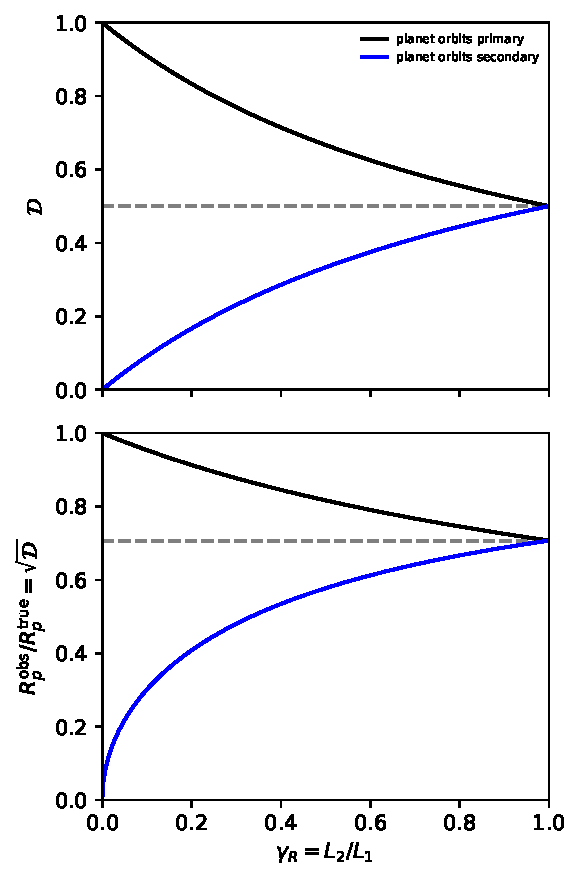
\includegraphics[scale=.9]{figures/observed_radii_vs_gammaR.pdf}
	\end{center}
	\caption{Dilution $\mathcal{D}$ and observed to true radius ratio 
	$\sqrt{\mathcal{D}}$ plotted against binary light ratio $\gamma_R$. This 
	illustrates	Eq.~\ref{eq:dilution}. The lower panel's horizontal line is at 
	$1/\sqrt{2}$.
	The implication is that if a detected planet orbits the secondary and you do 
	not know it, you cannot measure $R_p$ to better than $\approx 29\%$ 
	accuracy.
	Conversely, if it orbits the primary and you do not know it, you will get 
	the radius wrong by at most $\approx 29\%$.
	}
	\label{fig:rad_vs_gammaR}
\end{figure}

We could probably derive analytic expressions for all the terms between 
brackets in Eq.~\ref{eq:N_det_d_2}, completeness included.
I'm not yet convinced we need to -- we should get cancellations for
most of the questions we want to ask.

\subsubsection{Analytic completeness}
\texttt{todo, if necessary}
\subsubsection{Deriving ${\rm prob}(x_i)$}
\texttt{todo, if necessary}
\subsubsection{Number of detected planets}
\texttt{todo, if necessary}

\subsection{Astronomer A ignores binarity}

Just as in Sec.~\ref{sec:model_1}, Astronomer A
\begin{itemize}
\item has never heard about binary star systems.
\item has never heard about completeness corrections.
\item knows about geometric transit probabilities.
\end{itemize}

What occurrence rate does he derive for planets of radius $R_p$ and period $P$?

The answer is the same as in Sec.~\ref{sec:model_1},
\begin{equation}
\Gamma_{{\rm A}, R_p} = \frac{N_{\rm det,s}/f_{s,g}}{N_s + N_d}.
\end{equation}

However, now rather than planets detected in binary systems being perceived as 
a second population of planets with fixed radius $R_p \sqrt{\mathcal{D}}$, 
there will be an apparent spectrum of diluted radii, since $\mathcal{D}$ 
varies by system.
Writing the number of detections in double systems as a function of observed 
radius, $N_{\rm det,d}(R_p^{\rm obs})$, Astronomer A would derive an 
occurrence rate for this separate population of
\begin{equation}
\Gamma_{\rm A}(R_p^{\rm obs}) = \frac{N_{\rm det,d}(R_p^{\rm 
obs})/f_{s,g}}{N_s + N_d}.
\end{equation}
Note that this astronomer thinks these planets orbit single stars, 
and so miscomputes the geometric transit probability for the secondaries.

A more realistic question is ``what fraction of multiples have $\gamma_R$ 
smaller enough so that you'd still observe a radius close to the true one?''. 
We discuss this in Sec.~\ref{sec:close_enough}.

\subsection{Astronomer B counts host stars correctly}

Same as astronomer A above, except the denominator becomes $N_s + 2N_d$.

\subsection{Astronomer C counts host stars correctly and figures out diluted
radii}

In Sec.~\ref{sec:model_1}, Astronomer C only had to do high resolution 
imaging to measure $\gamma_R$ for each system. Since for $\gamma_R = 1$, the 
dilution is single-valued (Fig.~\ref{fig:rad_vs_gammaR}), this immediately 
told her the true planet radius (since the primary/secondary distinction was 
meaningless).

In Model \#2's universe, the dilution is double-valued for a given $\gamma_R$.
To correctly work out the diluted radii, Astronomer C now needs more than high 
resolution imaging -- she needs to resolve the stars during transit to 
discover which star the planet orbits.
She also needs to derive masses for the primaries and secondaries (to make the 
geometric transit probability correction).

Only after doing this does she find that all detected planets from this survey 
have radii $R_p$. She computes an occurrence rate
\begin{equation}
	\Gamma_{{\rm C},R_p} = 
	\frac
			{N_{\rm det,s}/f_{s,g} +
			  N_{\rm det,d1}/f_{d1,g} +
			  N_{\rm 	det,d2}/f_{d2,g}}
			{N_s + 2N_d}
\end{equation}

the closest yet to the true rate (Sec.~\ref{sec:true_rate}).


\subsection{Astronomer D counts host stars correctly, figures out diluted
radii, and accounts for completeness}

Same story as for Model \#1.
Now, they do injection recovery and derive correct estimates for their 
completeness functions about single stars $f_{s,c}$, the primaries of double 
star systems, $f_{d1,c}$, and the secondaries of double star systems 
$f_{d2,c}$.
They compute the respective single and binary 
occurrence rates
\begin{equation}
\Gamma_{t,s} = \frac{N_{\rm det,s}}{N_s f_{s,g} f_{s,c}},
\end{equation}
\begin{equation}
\Gamma_{t,d1} = \frac{N_{\rm det,d1}}{N_d f_{d1,g} f_{d1,c}},
\end{equation}
\begin{equation}
\Gamma_{t,d2} = \frac{N_{\rm det,d2}}{N_d f_{d2,g} f_{d2,c}}.
\end{equation}

With these in hand, they derive the overall occurrence rate
\begin{align}
\Gamma_{{\rm D}, R_p} 
&= \frac{
	N_{\rm det,s}/f_s + 
	N_{\rm det,d1}/f_{d1} +
	N_{\rm det,d2}/f_{d2}
	}
	{N_s + 2 N_d} \\
&= \frac{\Gamma_{t,s} N_s + (\Gamma_{t,d1} + \Gamma_{t,d2})N_d}
				{N_s + 2 N_d},
\end{align}
where $f_s \equiv f_{s,g}f_{s,c}, f_{d1} \equiv f_{d1,g}f_{d1,c}, 
f_{d2} \equiv f_{d2,g}f_{d2,c}$ for brevity.
Astronomer D's occurrence rate is the true occurrence rate (cf. 
Eq.~\ref{eq:true_occ_2}).


\subsection{Numerical verification}
\texttt{todo, if needed}


\subsection{Representative numbers for a few cases}

We have not given analytic expressions for the number of double star systems 
$N_d$ because even with simplified $M(L)$ relations, they are unwieldy.
However, we can ask similar numerical questions as from Sec.~\ref{sec:model_1}, 
and compare the answers.


\subsubsection{If we ignore binarity, for what fraction of detections do we
misclassify the radii?}

Ignoring binarity, we will detect $N_{\rm det,s}$ planets around single stars, 
and $N_{\rm det,d}$ planets around double stars. The latter set will be assumed 
to have radii $R_p \sqrt{\mathcal{D}}$, where $\mathcal{D}$ is the vector of 
dilutions appropriate for each binary star system.
The fraction of detections with misclassified radii can then be written
\begin{equation}
\frac{N_{\rm det,d}}{N_{\rm det,s} + N_{\rm det,d}} = \frac{1}{1+\alpha},
\end{equation}
for
\begin{equation}
\alpha \equiv 
\frac{ N_d (\Gamma_{t,d1} f_{d1} + \Gamma_{t,d2} f_{d2}) }{N_s \Gamma_{t,s} 
f_s},
\end{equation}
where $f_s \equiv f_{s,g}f_{s,c}, f_{d1} \equiv f_{d1,g}f_{d1,c}, 
f_{d2} \equiv f_{d2,g}f_{d2,c}$ for brevity.

% For the nominal G2V dwarf case of ${\rm BF}=0.45$, and the same distributions 
% used to generate 
% Figs.~\ref{fig:gammaR_distribn_vol_limited}~--~\ref{fig:gammaR_distribn_mag_limited},
% we found $N_d/N_s=0.59$.
% We are assuming $\Gamma_{t,d} / \Gamma_{t,s} = 1$.
% If we maintained the (incorrect) assumption that $f_{d,{\rm geom}} / f_{s,{\rm 
% 		geom}} = 1$, this would give a misclassification rate of 45\%. 
% 
% This latter assumption is wrong because although we are letting the occurrence 
% rate be the same across binary and single systems, our binary systems have 
% secondaries with varying masses. Thus they have varying radii.
% Taking [Demircan \& Kahraman 1991]'s empirical fit to eclipsing binary data,
% \begin{equation}
% R = 1.06 M^{0.945}
% \label{eq:mass_radius}
% \end{equation}
% for all the stars in our desired mass range ($M < 1.66M_\odot$, D\&K 1991's 
% stated bounds).
% For a zero eccentricity system, $f_{\rm geom}=R_\star/a$.
% Since $f_{d,{\rm geom}} = 0.5\times (f_{d1,{\rm geom}} + f_{d2,{\rm geom}})$, 
% \textit{i.e.} it is the average of the transit probabilities for both the 
% primary and secondary (d1 and d2), we can write (dropping the ``geom'' 
% subscript)
% \begin{align}
% \frac{f_d}{f_s} &= \frac{1}{2} \left(1 + \left(\frac{M_1}{M_{d2}}\right)^{1/3} 
% \frac{R_{d2}}{R_1}\right) \\
% &= \frac{1}{2} \left( 1 + q^{-1/3 + 0.945}\right).
% \end{align}
% 
% Computing it all out in a numerical simulation, the only thing that changes 
% analytically is that
% \begin{equation}
% N_d f_d \rightarrow \sum_{i=1}^{N_d} f_{d,i},
% \end{equation}
% so when considering the ratio $f_d/f_s$, we are in fact interested in
% \begin{equation}
% \frac{\langle f_d \rangle}{f_s} = \frac{\frac{1}{N_d} \sum_{i=1}^{N_d} 
% 	f_{d,i}}{f_s},
% \end{equation}
% where $f_{d,i}$ is the vector of geometric transit probabilities across all 
% systems.
% For the same numerical realization with $N_d/N_s = 0.59$, and using the mass 
% radius relation given by Eq.~\ref{eq:mass_radius}, I get $\langle f_d 
% \rangle / f_s = 0.84$ (smaller secondaries lead to a smaller average transit 
% probability in double star systems), for a radius misclassification rate of 
% $0.51$.


\texttt{The different secondary completeness matters here if proceeding 
analytically. Would be easier to do numerically.
Regardless, this is not the most interesting question right now.}

\subsubsection{If we ignore binarity, how wrong is our occurrence rate for
planets of radius $R_p$?}
\label{subsubsec:model2_A}

Write $\Gamma_{{\rm A,\ planets\ of\ }R_p} = \Gamma_{{\rm A,}R_p}$, 
and similarly for ${\rm D}$.
Just as in Model \#1, the answer to ``what is the relative difference between 
the occurrence rates derived by Astronomers D and A for planets of radius 
$R_p$?''
is simpler when we assume that Astronomer A has also derived a 
completeness, which we assume is the same as for Astronomer D in the single 
star case.
So Astronomer A now misclassifies planetary radii, and miscounts the total 
number of stars, but somehow knows his completeness for single 
stars. This is possible, because Astronomer A can correctly derive a 
completeness estimate and geometric transit probability for single stars only. 
For Astronomer $A'$ below, including the planets in binary star systems in the 
numerator introduces mistakes in the estimated completeness, and so the picture 
is more complicated.
Then
\begin{equation}
	\Gamma_{{\rm A}, R_p} = \frac{N_{\rm det,s}/(f_{s,g} f_{s,c})}{N_s + N_d}.
\end{equation}

The correction factor $X_\Gamma$ is
\begin{align}
X_\Gamma &=
\frac{\Gamma_{{\rm D},R_p}}{\Gamma_{{\rm A},R_p}} \\
&=
\frac{\Gamma_{t,s}N_s + (\Gamma_{t,d1} + 
	\Gamma_{t,d2})N_d}{N_s + 2N_d}  
\cdot 
\frac{N_s + N_d}{\Gamma_{t,s} N_s } \\
&= 
\frac{(1 + \beta (\Gamma_{t,d1}+\Gamma_{t,d2})/\Gamma_{t,s})(1 + 
	\beta)}{(1+2\beta)} 	\\
&=
(1 + \chi \beta )
\cdot 
\frac{1 + \beta}{1 + 2\beta }
\end{align} 
for
\begin{equation}
\beta \equiv N_d/N_s, \quad \chi \equiv 
(\Gamma_{t,d1}+\Gamma_{t,d2})/\Gamma_{t,s}.
\end{equation}

In the limit where the $R_p$ planet has the same occurrence rate about every 
host type regardless of its mass, $\chi=2$, and this simplifies to $X_\Gamma = 
1+\beta$.
This is same expression as what we found for Model \#1, but now the value of 
$\beta$ will be smaller in this model because of the 
smaller volume of searchable binary stars.
From numerics, we find $\beta = N_d/N_s = 0.59$, so the occurrence rate 
correction factor is $X_\Gamma(\chi=2) = 1.59$.

If we consider the opposite limit of the $R_p$ planet \textit{only} 
existing around single stars and the primaries of double star systems with 
equal occurrence, $\chi = 1$, and $X_\Gamma = (1 +\beta)^2 / (1+2\beta)$.
For $\beta = 0.59$, this gives $X_\Gamma(\chi=1) = 1.16$.
The true correction factor is somewhere between these two limits.



\subsubsection{What if we ignore binarity, but count derived planet radii that 
are ``close enough''?}
\label{sec:close_enough}

Let $x$ be the acceptable margin of error on the observed radius, so that we 
are interested in counting the number of planets detected with $R_p < R_p^{\rm 
obs} < (1\pm x) R_p$.
For Model \#2, since all planets have radius $R_p$, we only care about 
the smaller radius case, \textit{i.e.}, we want to count $R_p > R_p^{\rm 
	obs} > (1 - x) R_p$, for instance with $x=0.1$.

The diluted detections only occur in binary systems. The number of 
planets detected in double star systems with observed radius $R_p^{\rm obs}$ 
is
\begin{align}
N_{\rm det,d}(R_p^{\rm obs}) &= N_{\rm det, d1}(R_p^{\rm obs}) + 
								N_{\rm det, d2}(R_p^{\rm obs}) \\
&= \Gamma_{t,d1} f_{d1}(R_p^{\rm obs}) N_{d1}(R_p^{\rm obs})\  + \nonumber \\
&\quad\quad \quad\Gamma_{t,d2} f_{d2}(R_p^{\rm obs}) N_{d2}(R_p^{\rm obs}).
\end{align}
As always, the fractional terms $f_{di}$ for $i\in{1,2}$ encompass geometric 
and completeness corrections.
We're writing both them and the number of stars for which a given observed 
radius would be seen as functions of $R_p^{\rm obs}$.

To save on notational horribleness, write $R_p' \equiv \{(1-x) R_p < R_p^{\rm 
obs} < R_p\}$, in other words let $R_p'$ denote the set of planets that are 
observed in the desired radius range.

Then writing $N_{d1}(R_p')$, the number of double systems for which a $(R_p, 
P)$ planet would be observed in $R_p'$ if it orbiting the primary, is 
relatively straight-forward:
\begin{equation}
N_{d1}(R_p') = \int_{0}^{{\rm min}(1,\gamma_{R,u})} N_d(\gamma_R) 
\,{\rm prob}(\gamma_R) \,{\rm d}(\gamma_R),
\label{eq:N_d1}
\end{equation}
where the upper limit is set by equating the limiting radius $(1-x)R_p$ to the 
observed diluted radius $(1+\gamma_R)^{-1/2}R_p$, giving
\begin{equation}
\gamma_{R,u} \equiv \frac{x (2-x)}{(1-x)^2}.
\end{equation}
If $x > (1 - 2^{-1/2})$, bad things happen (cf. Fig.~\ref{fig:rad_vs_gammaR}), 
hence the need for the minimum.
Note that Eq.~\ref{eq:N_d1} is not an expression for the number of detected 
planets about primaries -- that quantity is expressed as $\Gamma_{t,d1} 
f_{d1}(R_p^{\rm obs}) N_{d1}(R_p^{\rm obs})$.

The analogous equation to Eq.~\ref{eq:N_d1} for $N_{d2}(R_p')$, the number of 
double systems for which a $(R_p, P)$ planet would be observed in $R_p'$ if it 
orbited the secondary, is
\begin{equation}
N_{d2}(R_p') = 
  \Bigg\{\begin{array}{lr}
  \int_{\gamma_{R,l}}^{1} N_d(\gamma_R)
  \,{\rm prob}(\gamma_R) \,{\rm d}(\gamma_R),\\ 
  \quad\quad\quad\quad\quad\quad\quad\quad x > 1 - 
  2^{-1/2}\\
  0, \quad\quad\quad\quad\quad\quad\quad x \leq 1 - 2^{-1/2} % lol
  \end{array}
\label{eq:N_Rp_secondary}
\end{equation}
where
\begin{equation}
\gamma_{R,l} \equiv \frac{(1-x)^2}{x (2-x)}.
\end{equation}
Eq.~\ref{eq:N_Rp_secondary} accounts for the fact that you cannot measure 
$R_p$ to better than $\approx 29\%$ if the planet orbits the secondary of an 
unidentified binary.
This was originally noted in Fig.~\ref{fig:rad_vs_gammaR}.

If we were forward-modelling, \textit{i.e.} if we actually wanted to compute 
$N_{\rm det,d}(R_p')$, we would also need to evaluate the total detection 
efficiency term $f_{d1}(R_p^{\rm obs})$, which is a product of the geometric 
transit probability and the fraction of signals of a given depth that are 
detectable.
We would need to integrate this product over the domain of allowable radii 
$R_p'$ to find the number of detected planets.

However, the procedure of estimating the geometric transit probability, as well 
as the completeness, is complicated by the errors that are introduced by 
including binary star systems that are thought to be single in the numerator.
These stars will have incorrectly estimated masses and radii, which influences 
both $f_c(R_p')$ and $f_g(R_p')$.

\texttt{If we ask the right question, we will not need to actually compute 
either term.}

Astronomer A misclassifies planetary radii, miscounts the total number of 
stars, and (incorrectly) estimates his completeness and geometric correction 
for ``single'' stars as a function of radius $f(R_p')$ (omitting a ``s'' 
subscript because the stars for which this incorrect occurrence rate are 
derived are not all single).
His occurrence rate for planets of radius \textit{near} $R_p$, \textit{i.e.} 
the set of planets with $\{ (1-x)R_p < R_p^{\rm obs} < R_p \}$, is
\begin{equation}
\Gamma_{{\rm A}, R_p'} = \frac{ (N_{\rm det,s} + N_{\rm det,d}(R_p')) 
/ f(R_p')   }{ N_s + N_d}.
\end{equation}

For him,
\begin{equation}
f(R_p') = f_g(R_p') f_c(R_p').
\end{equation}

Astronomer D, who had everything right, changes nothing.

The new correction factor is
\begin{align}
X_\Gamma &= \frac{\Gamma_{{\rm D},R_p}}{\Gamma_{{\rm A},R_p'} } \\
&=
\frac{1+\chi \beta}{1 + \xi}  \cdot 
\frac{1 + \beta}{1 + 2\beta},
\end{align}
for
\begin{equation}
\beta \equiv N_d/N_s, \quad \chi \equiv (\Gamma_{t,d1} + 
\Gamma_{t,d2})/\Gamma_{t,s},
\end{equation}
and
\begin{equation}
\xi \equiv \frac{N_{\rm det,d}(R_p')}{f(R_p')} \cdot \frac{1}{N_s 
\Gamma_{t,s}}.
\end{equation}
If we let $x < 1 - 2^{-1/2}$, for instance $x=0.1$, then $N_{d2}(R_p') = 0$. 
The expression for $\xi$ in this case becomes
\begin{align}
\xi &= \frac{N_{d1}(R_p')}{N_s} \cdot \frac{\Gamma_{t,d1}}{\Gamma_{t,s}} \cdot 
\frac{f_{d1}(R_p')}{f(R_p')} \\
&= \frac{N_{d1}(R_p')}{N_s} \cdot \frac{\Gamma_{t,d1}}{\Gamma_{t,s}} \cdot 
\frac{f_{g,d1}(R_p')}{f_g(R_p')}\cdot \frac{f_{c,d1}(R_p')}{f_c(R_p')},
\label{eq:chi_simplified}
\end{align}
provided that $x < 1-2^{-1/2}$.

We have now parametrized our ignorance.
The values that the latter two ratios of Eq.~\ref{eq:chi_simplified} take 
depend on what we assume Astronomer A' does to derive the stellar parameters 
for the systems that he thinks are singles but are in fact doubles.
For instance, assume he somehow observed the bolometric flux from every point 
on the sky, and used it with a distance to obtain single-star luminosities, and 
thus radii and masses.
His binary systems (thought to be singles) would be bluer than either component 
star is in reality.
On the main sequence, $\rho_\star$ decreases with increasing stellar radius, 
so $\rho_\star$ would be underestimated for all binaries.
Since $f_g \propto \rho_\star^{1/3}$, this means that $f_{g,d1}(R_p')/f_g(R_p') 
> 1$.
However, by the same token we can place an \textit{upper} bound on this ratio. 
In the worst case scenario a given star's luminosity is twice the individual 
star's luminosity. If $L\propto M^3 \propto R^3$, then the radius is 
over-estimated by at most a factor of $2^{1/3}$. Thus the density is 
underestimated by at most a factor of $2^{1/2}$, and $f_g(R_p')$ is 
underestimated by at most a factor of $2^{1/6}=1.12$. 

This begins to take us somewhere. The left-most term of 
Eq.~\ref{eq:chi_simplified} is bounded above by $\beta$. This is because 
$N_{d1}(R_p') \leq N_{d1} = N_d$.
If we assume $\Gamma_{t,d1} = \Gamma_{t,s}$, as we were doing 
anyway, then the product of the three left-most fractions must be less than 
$1.12\beta$.
The only thing standing in our way of an analytic upper bound to $\xi$ is the 
completeness fraction $f_{c,d1}(R_p')/f_c(R_p')$.
Note that over a fixed radius interval dilution will always 
yield a lower completeness fraction for double star systems than singles, so 
$f_{c,d1}(R_p') / f_{c,s}(R_p') \leq 1$.

For the completeness term, an argument that I don't wholly believe
is that
\begin{equation}
\frac{f_{c,d1}(R_p')}{f_c(R_p')} = \frac{f_{c,d1}(R_p')}{f_{c,s}(R_p')} \cdot
	\frac{f_{c,s}(R_p')}{f_{c}(R_p')} \lesssim 1 \cdot (1+\langle \gamma_R 
	\rangle)^3,
\end{equation}
where the first part of the inequality is obvious, but the second is by 
assuming it's $\lesssim f_{s,c}/f_{d,c}$, which might be wrong because of 
the radius dependence.

A way of making the estimate without deriving the actual 
completeness fractions, or even running numerics, is just to plot the error as 
a function of $\xi$. We do this in Fig.~\ref{fig:XGamma_vs_xi}, which 
shows that the correction factor varies from 0.6 to 1.6, depending on what 
fraction of secondaries you assume host planets.
\todo[inline]{I could run numerics for this to make the result more 
interesting.}

\begin{figure}[!t]
	\begin{center}
		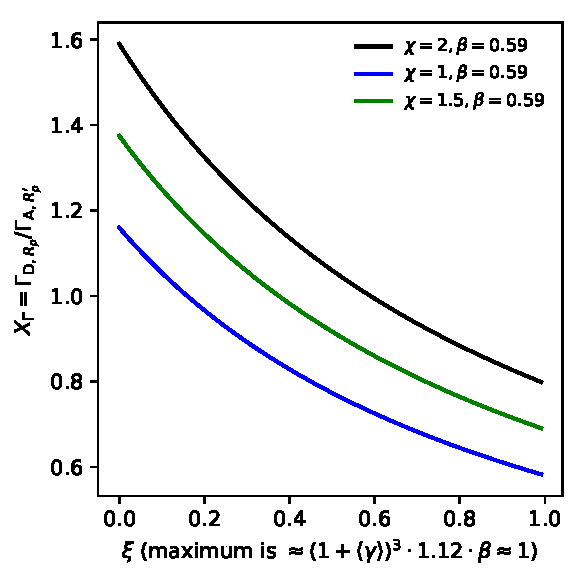
\includegraphics[scale=.8]{figures/XGamma_vs_xi.pdf}
	\end{center}
	\caption{\textit{Y axis}: correction factor for the astronomer who 
	ignores binarity but counts planetary radii that are ``close enough'' (A') 
	and the astronomer who knows everything (D).
	\textit{X axis}: $\chi$ as defined in Eq.~\ref{eq:chi_simplified}.
	}
	\label{fig:XGamma_vs_xi}
\end{figure}



\section{Model \# 3: A Synthetic {\it Kepler} Analog}
\label{sec:model_3}

\begin{figure}[!t]
	\begin{center}
		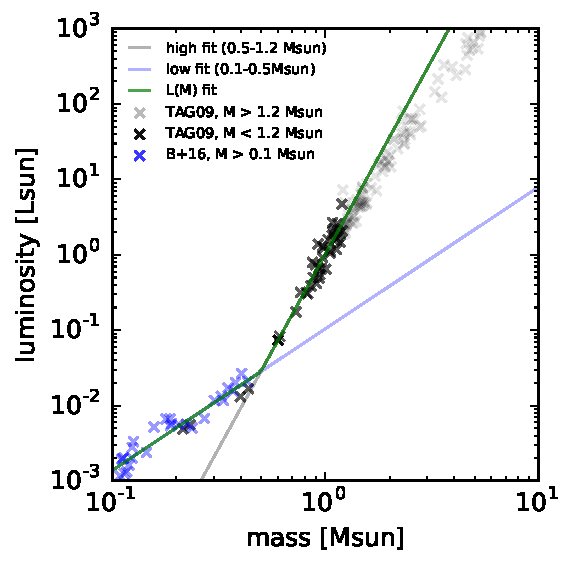
\includegraphics[scale=0.9]{figures/mass_luminosity.pdf}
	\end{center}
	\caption{Empirical fit to main sequence dwarf mass luminosity data compiled 
		from Torres et al. [2009] and Benedict et al. [2016]. The ``low fit'' is a 
		least squares fit to data from $0.1-0.5M_\odot$, and the ``high fit'' is 
		to 
		data above that, and below the Kraft break ($1.2M_\odot$).
		The $L(M)$ relation taken for numerics is the maximum 
		of the two fits. For analytics, we assume $L\propto M^{3.5}$.
	}
	\label{fig:mass_luminosity}
\end{figure}

If we assume every KIC star to be single, what order of magnitude of error do 
we make in occurrence rates estimated for planets of different sizes (and 
periods)?

We can attempt an answer with Monte Carlo simulations of something like the 
\kepler\ field. I say ``something like'' because the binarity properties of the 
\kepler\ field (or more specifically the stars selected in the KIC) are not 
known.
\todo[inline]{but it might be better to do something directly on the KIC's 
selected target stars, like what Ciardi did! The following is a good example, 
but at most it can ``suggest'' that a similar level of error has been made from 
the \kepler\ survey.

But it has MAJOR benefits compared to the GIC method.
It eliminates the need to simulate the biases of the KIC (since they're already 
baked in). The process of ``adding'' binaries to the KIC is the closest thing 
to REALITY, since in reality the KIC is missing binary companion information.
It BAKES IN all the real biases that come with mis-estimating stellar 
radii/masses when they are actually binaries (because it's already been done).
It also has literature precedent in Ciardi's work, so you don't need to cook up 
a crazy new procedure -- can just take his with the flaws baked in.

So this method is best if we care about what errors were made in Kepler/the KIC.
It's not as nice if we want something ``general''.
}

The plan is as follows:
\begin{itemize}
	\item Verify Galaxia can produce something resembling the KIC.
	\item Introduce binaries (Galaxia does not, by default, have any).
	\item Use Galaxia [Sharma et al 2010] to construct an analog of the KIC.
	\item Introduce a planet population.
	\item Numerically assess what occurrence rates would be derived, and 
	compare to previous sections.
\end{itemize}

\subsection{Verifying Galaxia can produce a KIC analog }

Galaxia [Sharma et al 2010] is a stellar population synthesis code for creating 
surveys of the Milky Way. It samples an assumed analytic distribution function. 
In other words, it assumes a number density of stars as a function of position, 
velocity, age, metallicty, and mass, from which it then samples to construct a 
``realistic'' stellar population.
The assumed model includes:
\begin{itemize}
	\item A metallicity distribution (log-normal),
	\item A velocity distribution (triaxial Gaussian),
	\item The stellar density and galactic components specified by Robin et al 
	[2003] (the Besan\c{c}on model) -- see Sharma et al [2010] Table 1. This 
	includes the IMF for a young and old thin disk, a thick disk, a spheroidal 
	component, a bulge component, as well as an ISM and dark halo. It also 
	includes the star-formation rate.
\end{itemize}

While this model of course lacks some detail, Sharma et al [2010] show that 
agreement with the volume-limited Hipparcos sample is probably good enough for 
our purpose of estimating the number of ``solar-like'' (by definition 
hereafter, $0.7 M_\odot < M_\star < 1.3 M_\odot$) stars in something like the 
\kepler\ field.

We then run the Galaxia in its ``circular survey'' mode, towards the direction 
of the \kepler\ field\footnote{galactic longitude 76.532562, galactic latitude 
13.289502.}. We apply the Schlegel, Finkbeiner et al [1999] extinction map when 
converting absolute to apparent magnitudes.

To verify the results are in reasonable agreement with the stars that actually 
exist in that direction, we compare the output with the KIC\footnote{From 
\url{http://archive.stsci.edu/kepler/kic.html}, we 
downloaded the 13.1 million row "|"-delimited gzipped ASCII file containing the 
complete Kepler Input Catalog (version 10).} [Brown et al 2011].
Following Sharma et al [2016, ApJ 822:15], for each catalog we selected all 
stars within $7.5^\circ$ of the center of the \kepler\ field, and with Sloan $r 
< 14$.
The KIC is complete to magnitudes fainter than $r=14$, so the comparison should 
not be affected by its completeness.

\begin{figure}[!t]
	\begin{center}
		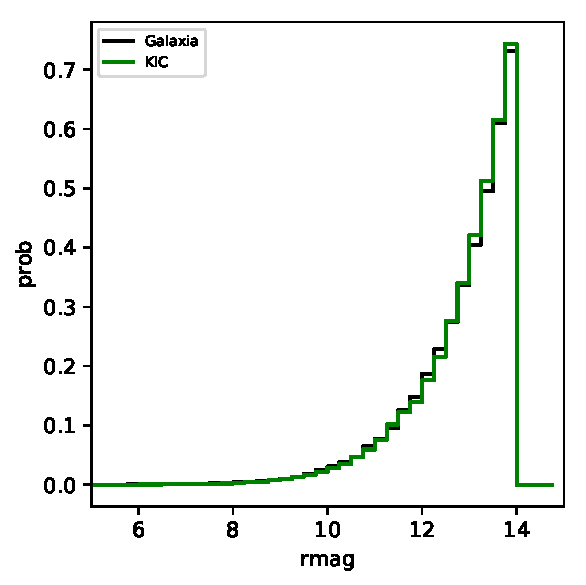
\includegraphics[scale=.8]{figures/rmag_distribn.pdf}
	\end{center}
	\caption{Probably density distributions of $r$ magnitude for $r<14$ stars 
	within $7.5^\circ$ of the center of the \kepler\ field, for Galaxia and the 
	KIC.	}
	\label{fig:rmag_distribn}
\end{figure}
\begin{figure}[!t]
	\begin{center}
		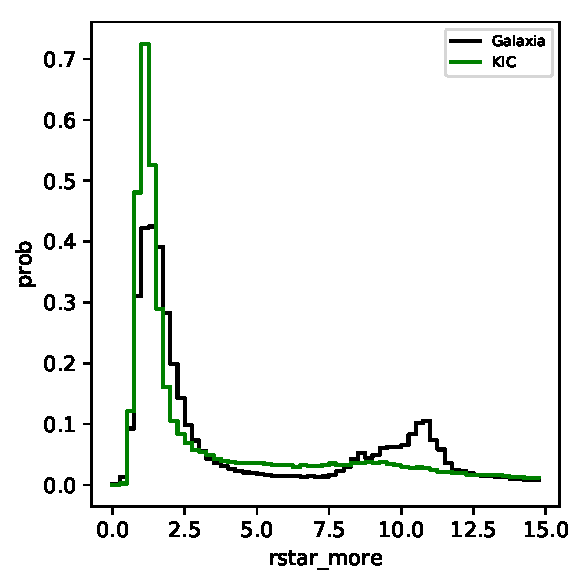
\includegraphics[scale=.8]{figures/rstar_more_distribn.pdf}
	\end{center}
	\caption{Same as Fig.~\ref{fig:rmag_distribn}, for $R_\star$.}
	\label{fig:rstar_more_distribn}
\end{figure}
\begin{figure}[!t]
	\begin{center}
		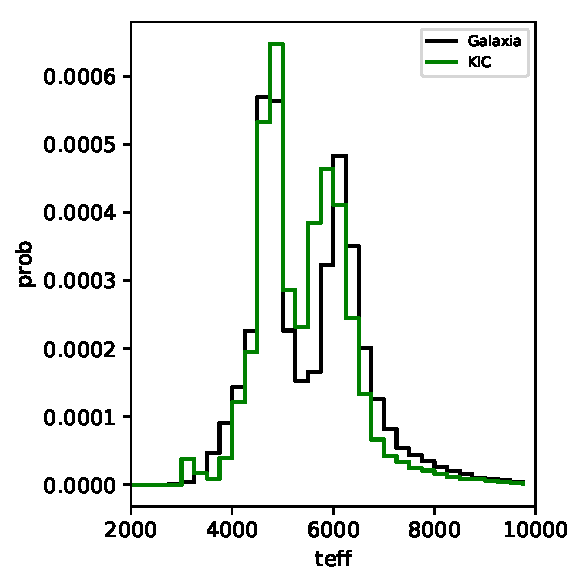
\includegraphics[scale=.8]{figures/teff_distribn.pdf}
	\end{center}
	\caption{Same as Fig.~\ref{fig:rmag_distribn}, for $T_{\rm eff}$.}
	\label{fig:teff_distribn}
\end{figure}

A few distributions are shown in 
Figs.~\ref{fig:rmag_distribn}-~\ref{fig:teff_distribn}.
From Fig.~\ref{fig:rmag_distribn}, we can see that the stellar counts as a 
function of Sloan $r$ magnitude are in close agreement with the KIC.
From Fig.~\ref{fig:rstar_more_distribn}, the KIC reports relatively more dwarf 
stars, and fewer giants than Galaxia does.
This is likely related to KIC's inability to distinguish between dwarfs and 
giants with only limited photometry -- although Brown et al [2011]'s idea of 
using a specific ``D51'' photometric band as a $\log g$ diagnostic was reported 
to have helped with this problem.
In Fig.~\ref{fig:teff_distribn}, we see something resembling the K dwarf desert 
again (5000K $\approx$ K3V dwarf).
Although there are a few slightly worrying discrepancies (notably in 
Fig.~\ref{fig:rstar_more_distribn}), we get the idea that Galaxia at least 
roughly resembles ``reality'' (inasmuch as the reported KIC parameters 
represent reality!).

\subsection{Introduce binaries}
\label{subsec:introduce_binaries}

By default, Galaxia does not include binaries.
However, from Fig.~\ref{fig:rmag_distribn}, we've seen that its number counts 
as a function of apparent magnitude are good.
So we assign binarity to the Galaxia stars as follows.
\begin{itemize}
	\item Assume a binary fraction ${\rm BF} = 0.44$ [Raghavan et al 2010].
	\item Ignore higher order multiples.
	\item If a star is drawn to be a binary:
	\subitem Its reported magnitude becomes a system magnitude.
	\subitem Draw the binary's mass ratio $q$ from the probability distribution 
	function for a magnitude limited survey, i.e. from 
	Fig.~\ref{fig:q_distribn_mag_limited}. This is sensible so long as the pdf 
	is independent of the primary's mass. We assume this to be the case over 
	$0.7-1.3M_\odot$\footnote{It was not immediately self-evident to me that 
	this distribution was the correct choice, since for fixed mass ratio as the 
	primary mass changes so does the detectable volume. However, as long as 
	${\rm prob}(q)$ is independent of the primary's mass, the average 
	distribution over all the possible detectable volumes will remain the 
	same.}.
	\subitem For $q \geq 5/7$, it turns out the above is sufficient information 
	to analytically specify the individual stellar masses, and thus 
	luminosities with the relation shown in Fig.~\ref{fig:mass_luminosity}.
	\subitem For $q < 5/7$, the individual stellar masses are not uniquely 
	specified\footnote{See the derivation of 2017/08/25. This is because of the 
	mass luminosity relation we specified, and the fact that we have $q$, and 
	$L_d$, but want individual masses, and individual luminosities.}. Thus for 
	this latter fraction of the population, we draw the 
	primary mass from the pdf of single star primary masses.
	\subitem With the individual masses known, use Eq.~\ref{eq:mass_radius} to 
	assign a radius to each star in the binary system.
\end{itemize}

Benefits of the above procedure include that it does not change Galaxia's 
star counts as a function of magnitude.
It produces the correct distribution of the mass ratio for the binaries in a 
magnitude limited sample, and thus a reasonable light ratio distribution. 

The drawbacks are that the individual component masses this procedure produces 
are not drawn from the same distribution throughout.
This might bias any subsequent synthetic transit survey.
From Fig.~\ref{fig:galaxia_scatter_masses}, it's likely not excessively 
important (it's more important to get the mass ratio and light ratio 
distributions correct).

In addition, the procedure produces a different mass-radius relation 
for stars in binary systems, vs. stars in single star systems.
This might also bias any subsequent synthetic transit survey.
The mass-radius relation for single stars comes from the Padova isochrones 
[Marigo et al 2008, Marigo \& Girardi 2007, Girardi et al. 2000, Bertelli et al 
1994] used in Galaxia.
Although Galaxia does not directly report radii, it reports luminosities and 
effective temperatures, from which we compute the radii.
The alternative choice would be to use the reported Galaxia masses with our 
Eq.~\ref{eq:mass_radius} to produce radius estimates.
This would produce consistency in the mass-radius relation, but would break $L 
= 4\pi R^2 \sigma T_{\rm eff}$ for single star systems.
The different mass-radius relations are shown in 
Fig.~\ref{fig:galaxia_mass_radius}.
Generally, it seems that the at a given mass, the stars in binary systems are 
biased to have slightly greater radii. (Ignoring the evolved stars).
However this is a small effect -- perhaps of order 10\% in the radius.
This will affect the transit depths in a synthetic transit survey, making it 
more difficult to detect planets around binaries.


\begin{figure}[!t]
	\begin{center}
		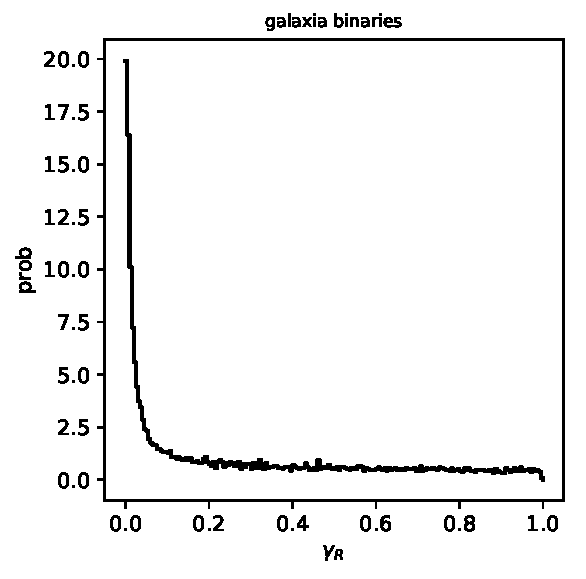
\includegraphics[scale=.8]{figures/galaxia_gammaR_distribn_mag_limited.pdf}
	\end{center}
	\caption{Light ratio distribution for the $r<17$ Galaxia sample discussed 
	in Sec.~\ref{subsec:introduce_binaries}.}
	\label{fig:galaxia_gammar_distribn}
\end{figure}
\begin{figure}[!t]
	\begin{center}
		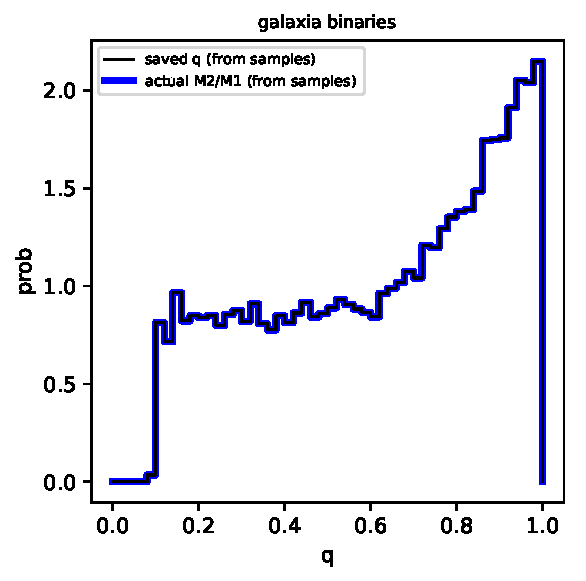
\includegraphics[scale=.8]{figures/galaxia_q_distribn_mag_limited.pdf}
	\end{center}
	\caption{Mass ratio distribution for the $r<17$ Galaxia sample discussed 
		in Sec.~\ref{subsec:introduce_binaries}.}
	\label{fig:galaxia_q_distribn}
\end{figure}
\begin{figure}[!t]
	\begin{center}
		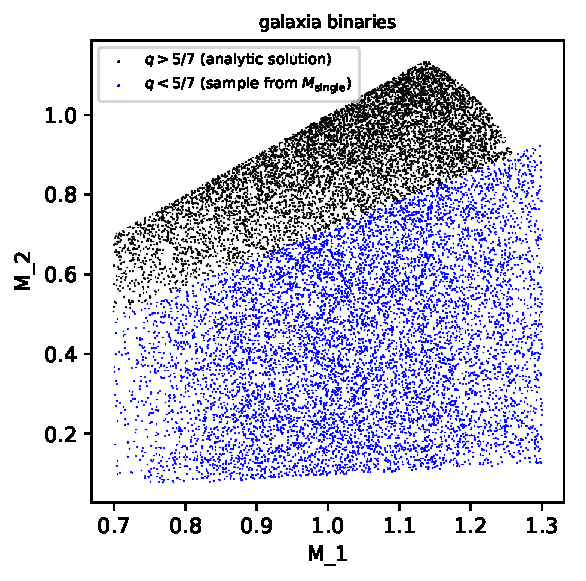
\includegraphics[scale=.8]{figures/galaxia_gammaR_scatter_masses.pdf}
	\end{center}
	\caption{Scatter plot of primary and secondary mass (solar units).}
	\label{fig:galaxia_scatter_masses}
\end{figure}
\begin{figure}[!t]
	\begin{center}
		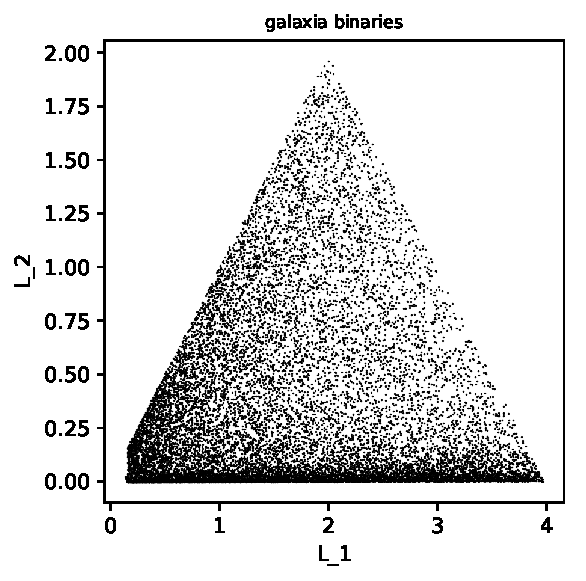
\includegraphics[scale=.8]{figures/galaxia_gammaR_scatter_luminosities.pdf}
	\end{center}
	\caption{Scatter plot of primary and secondary luminosity (solar units).}
	\label{fig:galaxia_scatter_luminosities}
\end{figure}
\begin{figure}[!t]
	\begin{center}
		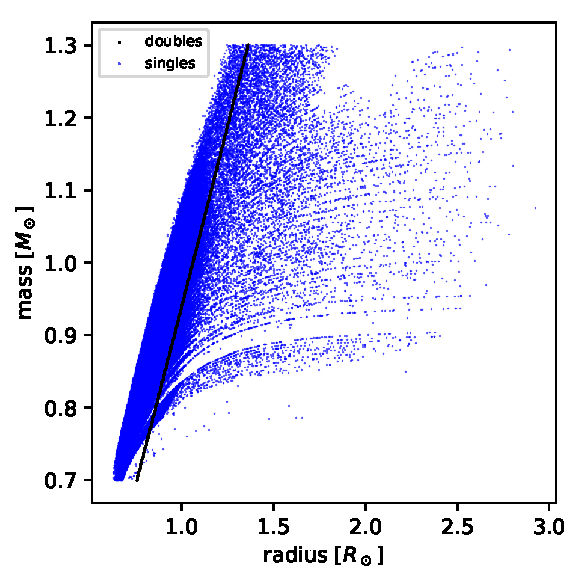
\includegraphics[scale=.8]{figures/galaxia_compare_mass_radius.pdf}
	\end{center}
	\caption{Scatter plot of mass vs radius for singles and binaries. For 
	binaries, different points are shown for the primary and secondary of a 
	given system. Only points with $0.7<M_\star/M_\odot<1.3$ are selected.}
	\label{fig:galaxia_mass_radius}
\end{figure}


\subsection{Using Galaxia to construct a KIC analog}

With glowing confidence, we then proceed to construct a KIC analog as follows.
We take all Galaxia stars within 7.5 degrees of the center of the \kepler\ 
field, and take stars with $r<17$.
\todo[inline]{a different magnitude cut, e.g. $r<16$, might matter?}
This is now beyond where the KIC is complete, so direct comparisons of 
distributions with the KIC will be confused.
We then apply an analog of the prioritization scheme used by the \kepler 
mission to select target stars, described by Batalha et al [2010]'s Table 1. 

For each star, we compute the minimum detectable planet radius at three 
semimajor axes: (1) the inner radius of the so-called ``habitable'' zone,
\begin{equation}
a_{\rm HZ} = 0.95\, {\rm AU} \left(\frac{L}{L_\odot}\right)^{1/2},
\end{equation}
(2) $0.5 a_{\rm HZ}$, and (3) $5R_\star$. We make the same assumptions as 
Batalha et al [2010] did about the transit duration. We assume a noise model of 
pure shot noise, rather than using any CDPP estimates.
We then apply the Batalha et al [2010] Table 1 prioritization, except 
that we use SDSS $r$ magnitudes instead of Kepler $Kp$ magnitudes.
The rankings are shown in Fig.~\ref{fig:batalha_table_1}.
We get similar (within a factor of two) counts as they did towards the end of 
the table, though at the beginning we seem to have fewer stars\footnote{I 
suspect this is because of the slightly different noise calculation -- and 
perhaps Batalha using $N_{\rm sample}$ rather than just counting photons 
matters}.

\begin{figure}
	\begin{center}
		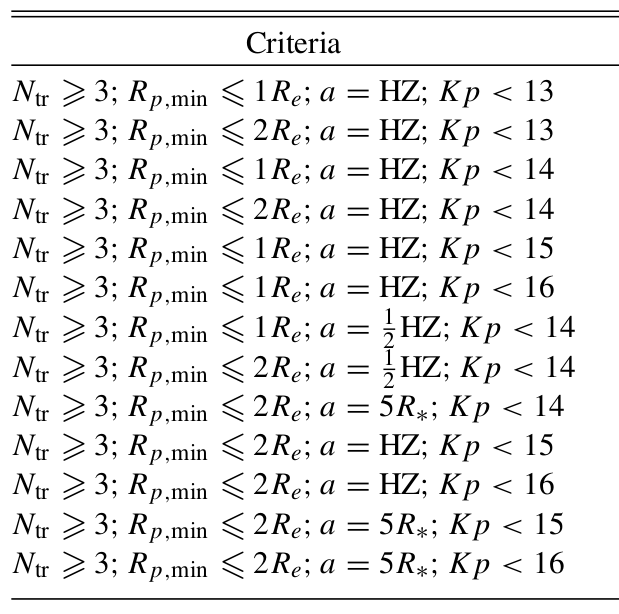
\includegraphics[scale=0.3]{figures/batalha_2010_table_1.png}
	\end{center}
	\caption{Prioritization applied by Batalha et al [2010], from whom I 
	copy-pasted this Table. I did the same, but using $r$ magnitudes instead of 
	$Kp$.}
	\label{fig:batalha_table_1}
\end{figure}
\begin{figure}[!t]
	\begin{center}
		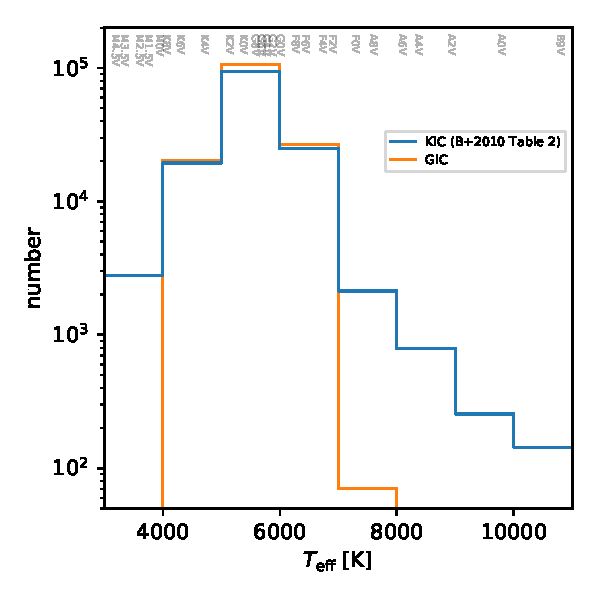
\includegraphics[scale=0.8]{figures/KIC_vs_GIC_teff_distribn.pdf}
	\end{center}
	\caption{Effective temperature distribution of the stars in our synthetic 
		Kepler input catalog analog -- the Galaxia input catalog.
		Note that the effective temperatures of binary star systems in the GIC 
		are 
		intentionally wrongly estimated, as if they were single star systems.
		The listed $T_{\rm eff}$ to spectral type correspondence is from 
		Mamajek's tables.
	}
	\label{fig:KIC_vs_GIC_teff_distribn}
\end{figure}


Note that, since we assigned binarity to Galaxia stars, applying the Batalha et 
al [2010] prioritization procedure requires estimating \textit{incorrect} 
single star parameters for what are really binary star systems!
We do this by keeping the total system luminosity, inverting 
Fig.~\ref{fig:mass_luminosity} to find an incorrect mass, and then applying 
Eq.~\ref{eq:mass_radius} to get an incorrect radius.
We can then calculate the minimum detectable planet radius as
\begin{equation}
R_{p,{\rm min}} = \left(\frac{7.1 \sigma_{\rm tot}}{r}\right)^{1/2} R_\star,
\label{eq:min_det_radius}
\end{equation}
for $r=1$ the dilution that we ignore, and
\begin{equation}
\sigma_{\rm tot} \equiv {\rm N} = (F_\gamma^{\rm N} A N_{\rm tra} T_{\rm 
dur})^{-1/2}
\end{equation}

In applying the prioritization, we omit the latter two priority classes of 
Fig.~\ref{fig:batalha_table_1}, to obtain a catalog of 152682 stellar systems, 
which we hereafter refer to as the \textit{Galaxia Input Catalog (GIC)}.
We compare the effective temperature distribution of the GIC with 
that of the KIC, reported by Batalha et al [2010] Table 2, in 
Fig.~\ref{fig:KIC_vs_GIC_teff_distribn}. Evidently, the GIC is 
dominated by sun-like stars, in a very similar manner to the exoplanet target 
stars of the KIC.


\subsection{Introduce a planet population}

As in Sec.~\ref{sec:model_2}, we allow for three different occurrence rates: 
$\Gamma_{t,s}$, the fraction of stars in single systems with a planet of radius 
$R_p$ and orbital period $P$, and also $\Gamma_{t,d1}$ and $\Gamma_{t,d2}$ for 
the fraction per sun-like primary and secondary (respectively) of double star 
systems with a planet of $(R_p, P)$.

We then randomly select which stars get a planet, and using the true stellar 
masses and radii compute the corresponding impact parameters for the planets as
\begin{equation}
b = \frac{a}{R_\star} \cos i, \quad \cos i \sim \mathcal{U}(0,1).
\end{equation}
Any planet with $|b| < 1$ is transiting, and has its transit duration evaluated 
as
\begin{equation}
T_{\rm dur} = 13\,{\rm hr} \left(\frac{P}{{\rm yr}}\right)^{1/3} 
\left(\frac{\rho_\star}{\rho_\odot}\right)^{-1/3} \sqrt{1 - b^2},
\end{equation}
which assumes circular orbits.

\subsection{Run the survey}
We run the following survey:
$A = 0.708\,{\rm m}^2$ (\kepler\ effective area), $T_{\rm obs} = 20\,{\rm 
years}$ (to detect more Earth-like planets than \kepler\ did), and $x_{\rm min} 
= 7.1$, the same signal to noise threshold as \kepler.

For simplicity, we assign a $r$ band zero point of $10^6\,{\rm ph/s/cm}^2$ to 
correspond to an $r=0$. We use this to compute the observed 
photon number fluxes for every system, regardless of whether it has a planet.
We then compute the signal to noise distribution of transit events, and the 
number of detections, according to Eq.~\ref{eq:snr_ivory_tower}.


\subsection{Numerically assess what occurrence rates would be derived, and 
	compare to previous models}

\subsubsection{If we ignore binarity, how wrong is our occurrence rate for 
	planets of radius $R_p$?}

This is similar to what we did in Sec.~\ref{subsubsec:model2_A}, with the 
exception that we need to specify the calculation more precisely.

Specifically, our ``Astronomer A'' in this case will estimate an occurrence 
rate for planets of radius $R_p$ and orbital period $P$ as
\begin{equation}
\Gamma_{{\rm A}, R_p} = \frac{N_{\rm det,s}}{Z},
\label{eq:rate_A}
\end{equation}
for
\begin{equation}
Z \approx (N_s + N_d) \frac{1}{J} \sum_{j=1}^{J} Q_j,
\end{equation}
for $Q_j$ the total detection efficiency, indexed over single and double 
systems, given as the product of the geometric transit probability and the 
system-specific completeness:
\begin{equation}
Q_j \equiv f_g^{(j)} f_c^{(j)}.
\end{equation}

Keep in mind that for Astronomer A, we need to compute the 
\textit{incorrect} transit probability for double star systems (since 
Astronomer A is assuming that they are single stars).

To evaluate the system-level completeness, we assume that Astronomer A performs 
something equivalent to perfect injection-recovery.
For a stellar system with known properties (stellar and planetary), and a 
perfectly known noise model, the probability of detection is a binary function: 
either ${\rm S/N} > {\rm (S/N)_{min}}$, or it is not\footnote{There are 
probabilities involved if we allow for any uncertainty in the parameters, but 
this is too complicated for our current goal.}.
So we compute $f_c^{(j)}$ as Astronomer A would: an array (over star systems) 
of zeros wherever the $(R_p,P)$ planet could not be detected, and ones where it 
could.
We then evaluate the total detection efficiency $Q_j$ for each system, and 
compute the occurrence rate as in Eq.~\ref{eq:rate_A}.
The resulting occurrence rates are only slightly smaller than those in 
Sec.~\ref{subsubsec:close_enough} discussed below and shown in 
Fig.~\ref{fig:error_vs_occrate}.

\subsubsection{What if we ignore binarity, but count planets whose derived 
radii are ``close enough'' to $R_p$?}
\label{subsubsec:close_enough}

As in Sec.~\ref{sec:model_2}, we now count planets with observed radii from 
$(1-x)R_\oplus < R_p^{\rm obs} < R_\oplus$. We'll use $x=0.1$, but it can be 
whatever we want.
The occurrence rate in this case will be
\begin{equation}
\Gamma_{A,R_p'} = \frac{N_{\rm det,s} + N_{\rm det,d}(R_p')}{Z'},
\end{equation}
for
\begin{equation}
Z' \approx (N_s + N_d) \frac{1}{J} \sum_{j=1}^{J} Q_j',
\end{equation}
where the geometric transit probability is the same as before, but the 
system-specific completeness is now a function of the desired radius interval:
\begin{equation}
Q_j' = f_g^{(j)} f_c^{(j)}(R_p').
\end{equation}
There are three possible cases for the completeness, specified by the minimum 
detectable planet radius $R_{p,{\rm min}}$ (computed according to 
Eq.~\ref{eq:min_det_radius}):
\begin{align}
f_c^{(j)}(R_p') &= 
\Bigg\{\begin{array}{lr}
1 & {\rm\ if\ }R_{p,{\rm min}}>R_p,\\
0, & {\rm\ if\ }R_{p,{\rm min}}<(1-x)R_p,\\
\frac{R_p - R_{p,{\rm min}}}{R_p - (1-x)R_p}, &{\rm otherwise}.
\end{array}
\label{eq:completeness_close_enough}
\end{align}
The latter term above is the case in which the minimum detectable planet 
radius happens to be between $(1-x)R_p$ and $R_p$. In that case the 
completeness becomes the fraction of planets in that interval that would be 
detected.
Assuming a uniform prior for the planet radius distribution $R_p \sim 
\mathcal{U}((1-x)R_p, R_p)$, this becomes the expression given in 
Eq.~\ref{eq:completeness_close_enough}.

These occurrence rates can then be compared to the ``true occurrence rate'' 
derived by the all-knowing Astronomer D:
\begin{equation}
\Gamma_{{\rm D}, R_p} = \frac{\Gamma_{t,s} N_s + (\Gamma_{t,d1} + 
						\Gamma_{t,d2})N_d}{N_s + 2 N_d}.
\end{equation}
A note in passing: the more information-rich parameters for Astronomer D to 
report would be $(\Gamma_{t,s}, \Gamma_{t,d1}, \Gamma_{t,d2})$, rather than 
$\Gamma_{{\rm D}, R_p}$. But I digress.

Similar to Fig.~\ref{fig:XGamma_vs_xi}, Fig.~\ref{fig:error_vs_occrate} 
shows that the magnitude of the correction needed by the $\Gamma_{{\rm 
A},R_p'}$ estimate depends strongly 
on the fraction of secondaries that are assumed to host the $(R_p, P)$ planets.
The simplest assumption is that the occurrence rate is the same for all solar 
type stars: any ``Sun-like'' ($0.7<M_\star/M_\odot<1.3$) star hosts planets at 
the ``true rate'' $\Gamma_t$, and any other mass of star does not.
Given how we have defined the GIC, this means that all single stars and 
primaries of double star systems are sun-like. The fraction of Sun-like 
secondaries in this case is 37.4\% of all secondaries.
Reading the appropriate value off Fig.~\ref{fig:error_vs_occrate}, this 
corresponds to $\Gamma_{\rm D} = 1.39 \Gamma_{\rm A'}$.
This gives a relative percentage error of $\delta\Gamma_{{\rm D},R_p} \equiv 
(\Gamma_{\rm A,R_p'} - \Gamma_{\rm D,R_p}) / \Gamma_{\rm D,R_p} = -28\%$.


\begin{figure}[!t]
	\begin{center}
		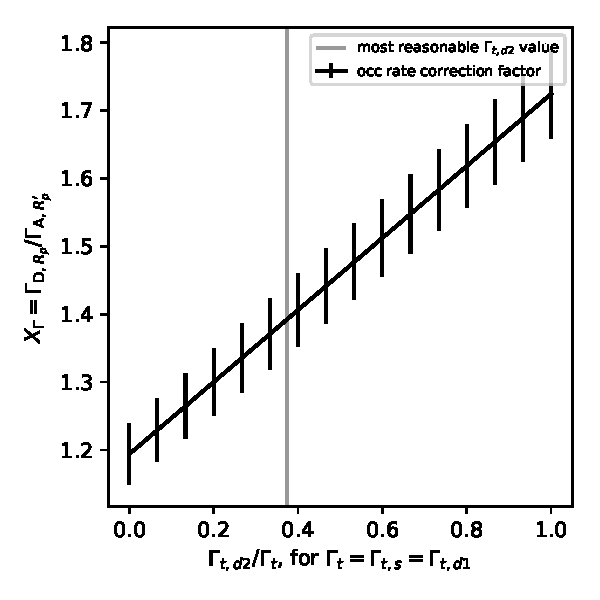
\includegraphics[scale=0.8]{figures/error_vs_occrate.pdf}
	\end{center}
	\caption{ The ``most reasonable'' $\Gamma_{t,d2}$ value is obtained by 
	assuming that the occurrence rate of $(R_p, P)$ planets is the same for all 
	solar type stars, and zero otherwise.
	This applies most immediately to the question of Earth-like planets around 
	Sun-like stars.
	}
	\label{fig:error_vs_occrate}
\end{figure}

\end{comment}



% \begin{comment}
% \subsection{How many stars are in the sample?}
% \subsection{How many planets are in the sample?}
% \subsection{What is the true occurrence rate?}
% \subsection{How many planets are detected?}
% \subsubsection{Analytic completeness}
% \subsubsection{Deriving ${\rm prob}(x_i)$}
% \subsubsection{Number of detected planets}
% \subsection{Astronomer A ignores binarity}
% \subsection{Astronomer B counts host stars correctly}
% \subsection{Astronomer C counts host stars correctly and figures out diluted
% radii}
% \subsection{Astronomer D counts host stars correctly, figures out diluted
% radii, and accounts for completeness}
% \subsection{Numerical verification}
% \subsection{Representative numbers for a few cases}
% \subsubsection{If we ignore binarity, for what fraction of detections do we
% misclassify the radii?}
% \subsubsection{If we ignore binarity, how wrong is our occurrence rate for
% planets of radius $R_p$?}
% \subsubsection{If we ignore binarity, but allow derived planet radii to be
% ``close enough'', how do we do?}
% 
% \end{comment}


\newpage

%\begin{thebibliography}{}


%\end{thebibliography}

\end{document}
